\section{Design drawings}
In this chapter, the extracts from the design drawings relevant to this Thesis are presented. The general notes on the materials and load combinations are given in Section \ref{app:general_notes}. The cross-sections of the different segments are presented in Section \ref{app:cross_sections}. The weight of the bridge is estimated from the summary of quantities in Section \ref{app:weight}. Ultimately, a summary of the final design verifications is given in Section \ref{app:design_verifications}. The values refer to the American units \SI{}{ft}, \SI{}{in}, \SI{}{kip}, \SI{}{kip ft} and \SI{}{ksi}. The general plan is shown in Fig. \ref{fig:general_plan}.
\begin{figure}[H]
    \centering
    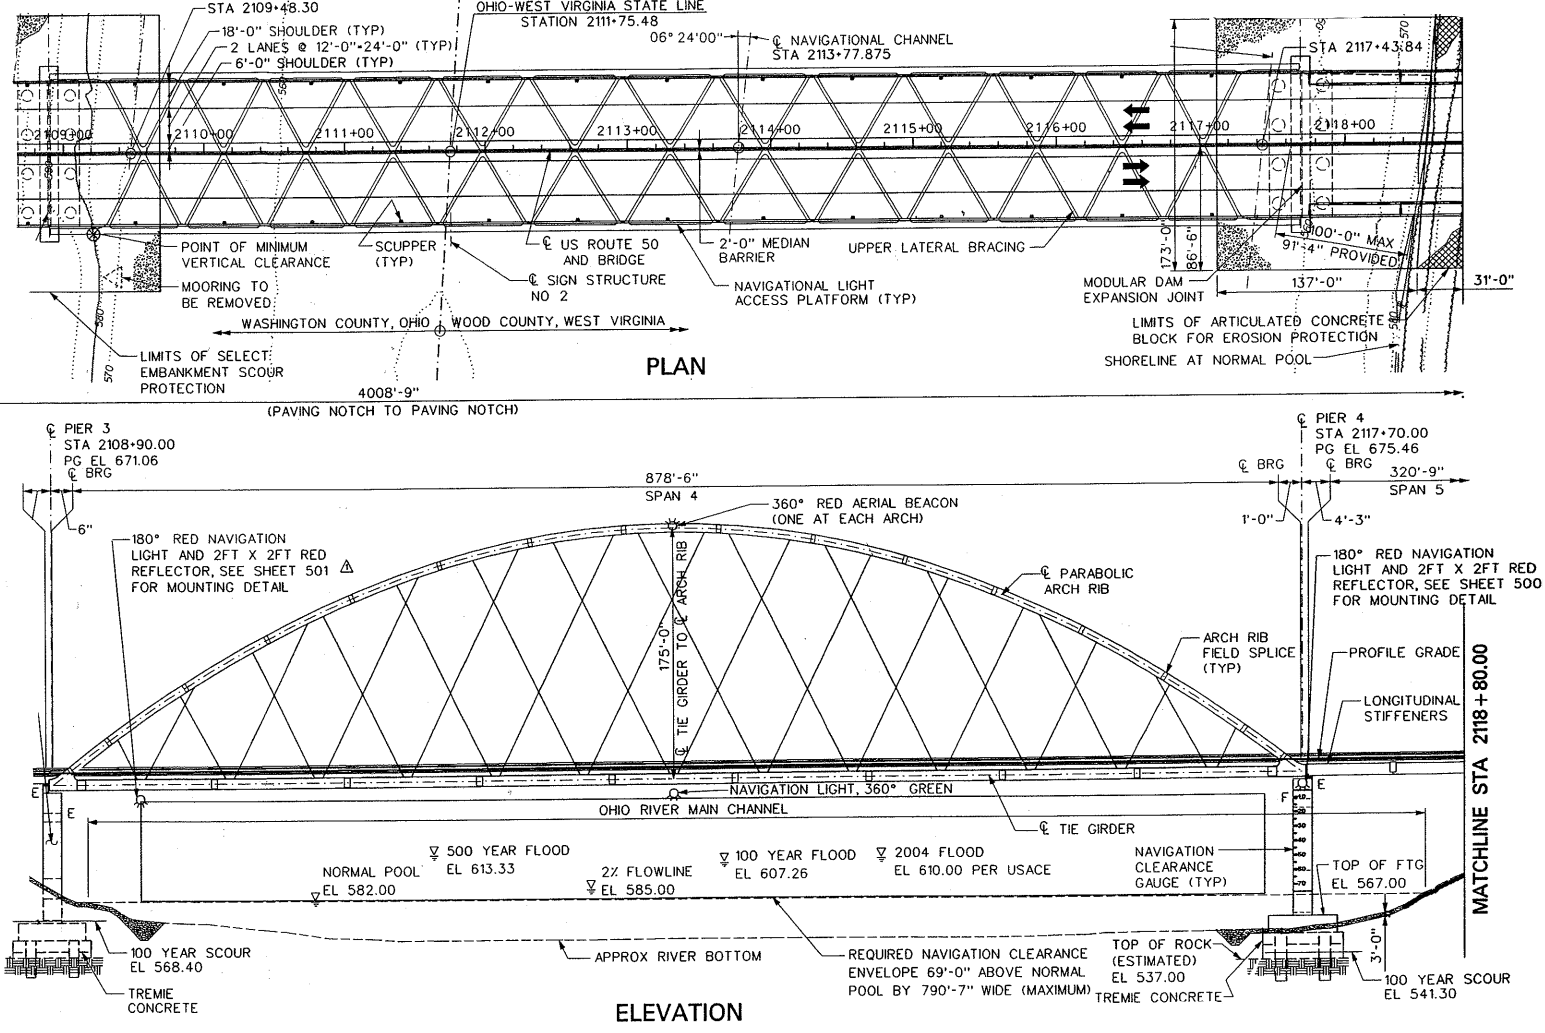
\includegraphics[width=\textwidth]{overleaf/Appendix/Design drawings/General Plan.png}
    \caption{General plan}
    \label{fig:general_plan}
\end{figure}

\subsection{General notes} \label{app:general_notes}
The general notes on the materials, the hanger resistance factors and the load combinations for cable loss and tie fracture are presented in Figs. \ref{fig:materials} to \ref{fig:hanger_load_combination}.
\begin{figure}[H]
    \centering
    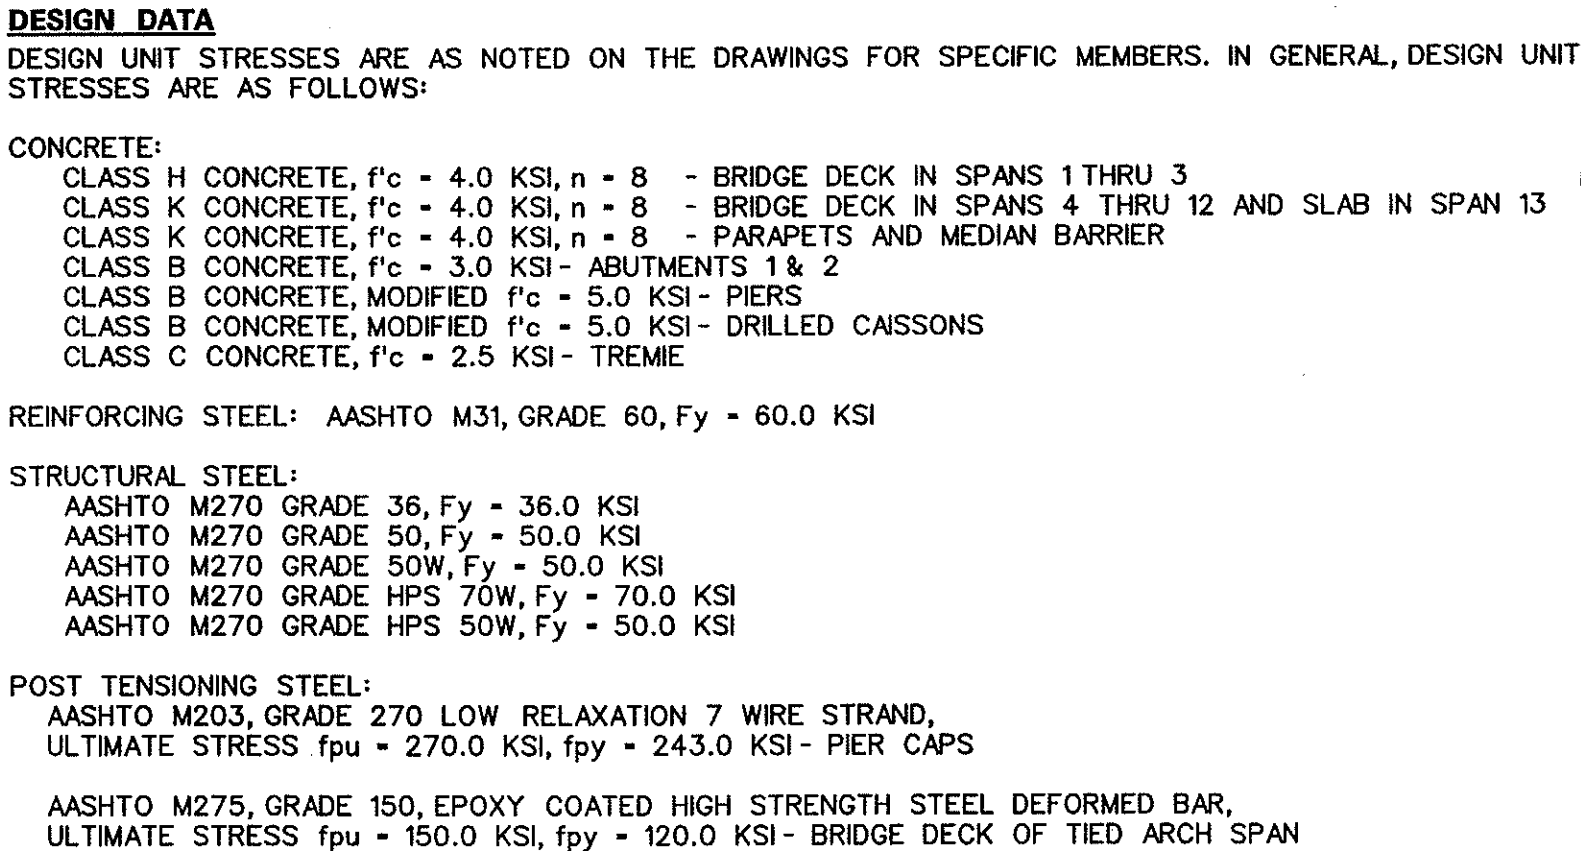
\includegraphics[width=0.65\textwidth]{overleaf/Appendix/Design drawings/Material design data.png}
    \caption{Material design data}
    \label{fig:materials}
\end{figure}
\begin{figure}[H]
    \centering
    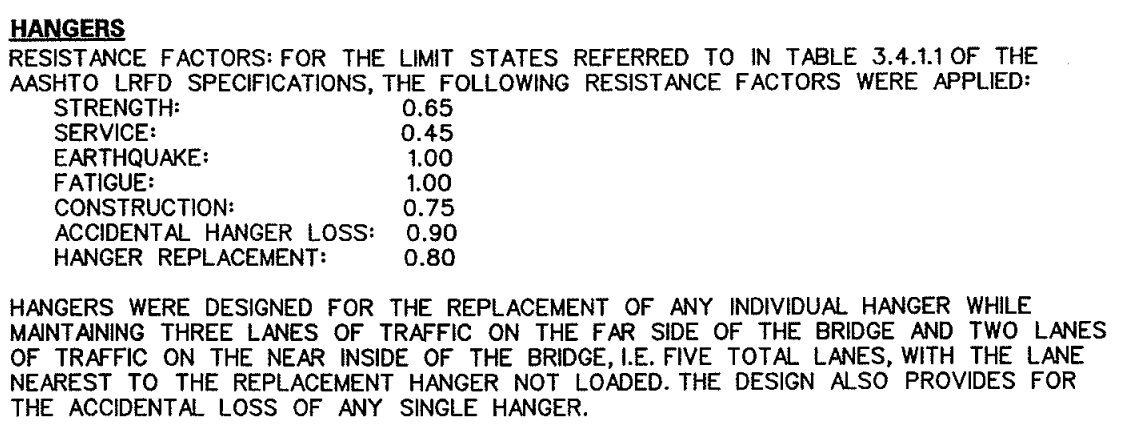
\includegraphics[trim={0 0.9cm 0 0cm},clip, width=0.6\textwidth]{overleaf/Appendix/Design drawings/Hanger resistance factor.PNG}
    \caption{Hanger resistance factors}
\end{figure}
\begin{figure}[H]
    \centering
    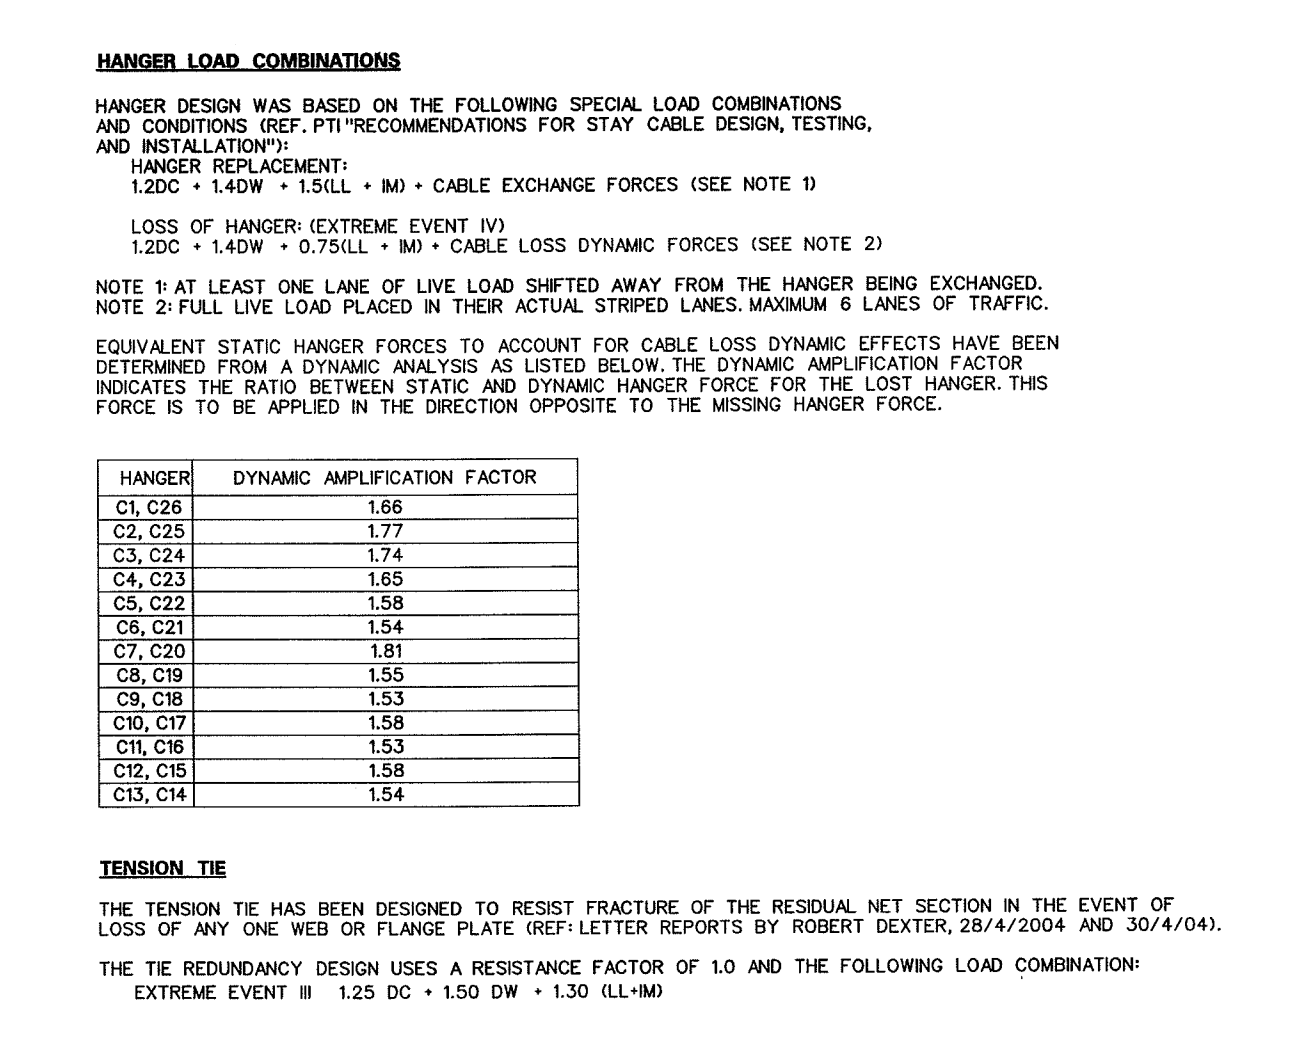
\includegraphics[trim={0 0.5cm 0 0.7cm},clip, width=0.69\textwidth]{overleaf/Appendix/Design drawings/Hanger load combination.png}
    \caption{Load combinations for extreme events and dynamic amplification factors}
    \label{fig:hanger_load_combination}
\end{figure}
%\begin{figure}[H]
%    \centering
%    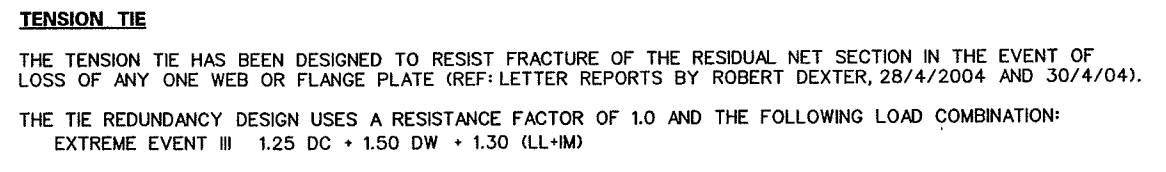
\includegraphics[width=0.8\textwidth]{overleaf/Appendix/Design drawings/Tension tie.PNG}
%    \caption{Tie fracture load combination}
%    \label{fig:tie_fracture_loads}
%\end{figure}

\subsection{Cross-sections} \label{app:cross_sections}
In this section, the cross-sections are introduced. The dimensions and the resistances were taken from the design verification tables, which are shown in Section \ref{app:design_verifications}. The three characteristic cross-sections in the field are shown in Figs. \ref{fig:cs_arch} to \ref{fig:cs_cable}. 
\begin{figure}[H]
\centering
\begin{subfigure}{0.33\textwidth}
    \centering
    \vspace*{0.68cm}
    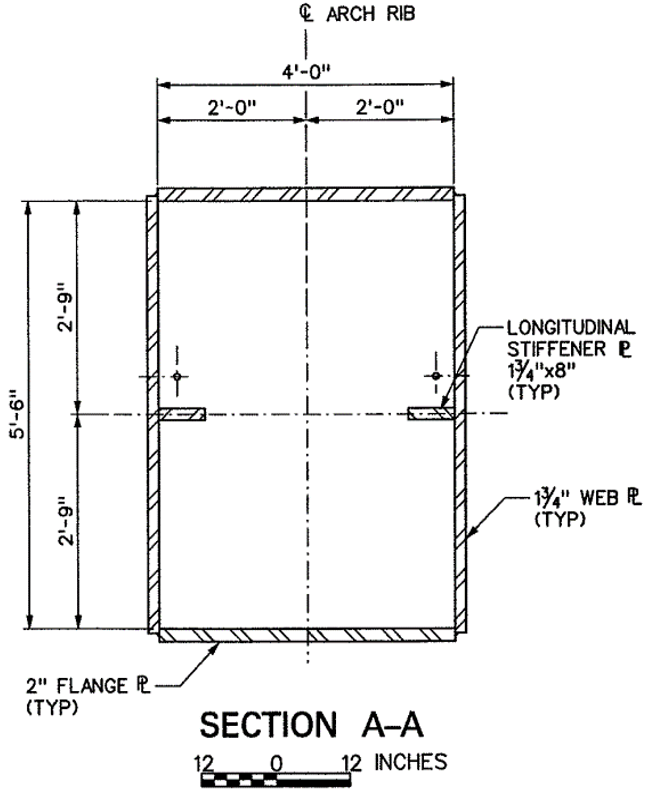
\includegraphics[width=0.8\textwidth]{overleaf/Appendix/Pictures/arch_3.PNG}
    \vspace*{0.68cm}
    \caption{Arch rib}
    \label{fig:cs_arch}
\end{subfigure}%
\begin{subfigure}{.33\textwidth}
    \centering
    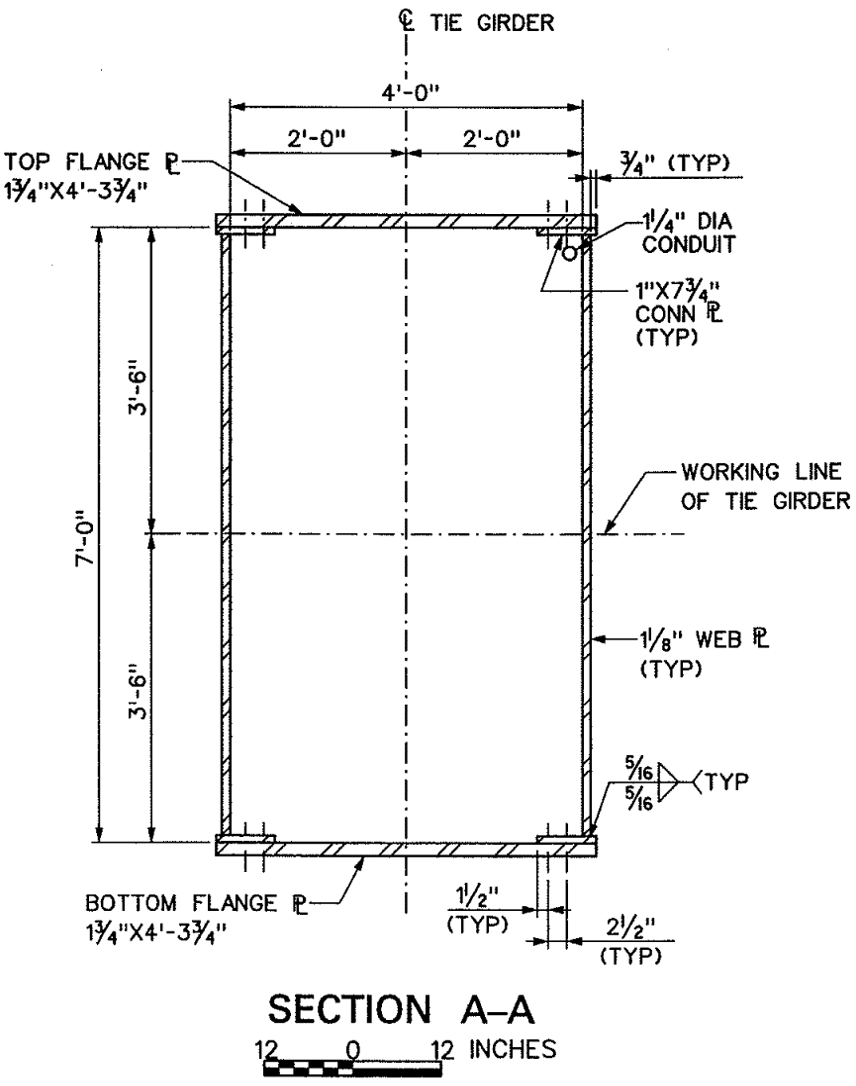
\includegraphics[width=\textwidth]{overleaf/Appendix/Pictures/tie_3.PNG}
    \caption{Tie girder}
    \label{fig:cs_tie}
\end{subfigure}%
\begin{subfigure}{.33\textwidth}
    \centering
    \vspace*{1.35cm}
    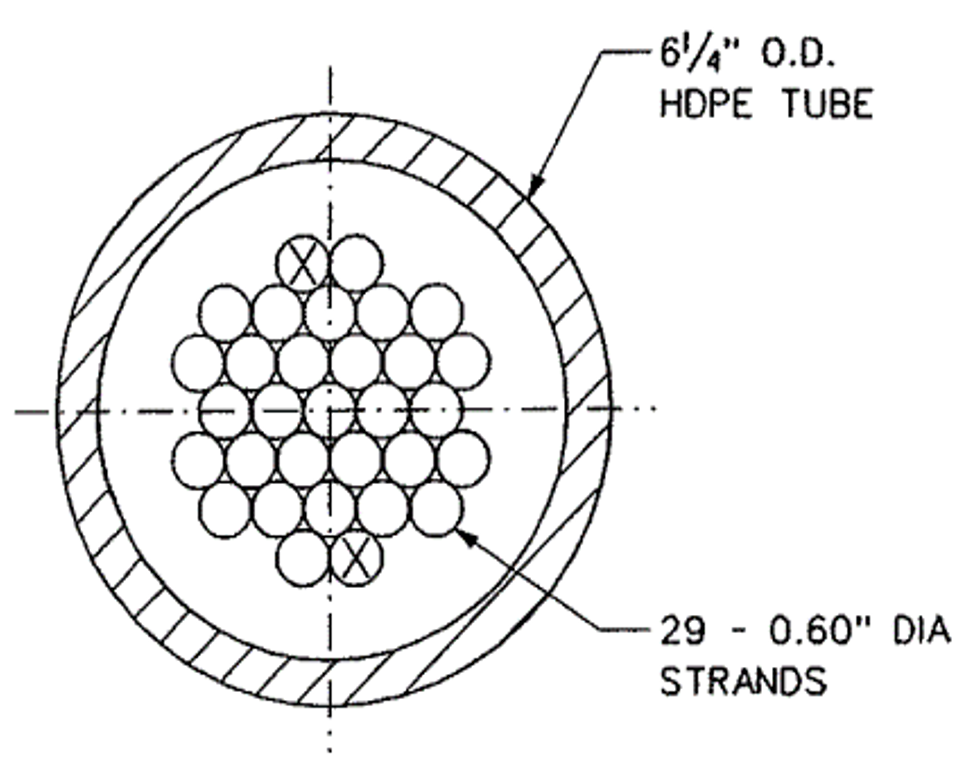
\includegraphics[width=0.9\textwidth]{overleaf/Appendix/Pictures/cable_3.PNG}
    \vspace*{1.35cm}
    \caption{Cable}
    \label{fig:cs_cable}
\end{subfigure}\caption{Cross-sections}
\label{fig:cross_sections}
\end{figure}

The cross-sectional properties are shown in Tables \ref{tab:cs_arch} to \ref{tab:cs_cable}.

\begin{table}[H]
\centering
\resizebox{0.85\textwidth}{!}{%
\begin{tabular}{lcccc}
\hline
Cross-Section          & Arch 1             & Arch 2             & Arch 3             &            \\ \hline
Flange width           & 1.219              & 1.219              & 1.219              & {[}m{]}    \\
Flange thickness       & 0.051              & 0.051              & 0.051              & {[}m{]}    \\
Subflange width        & 1.715              & 1.715              & 1.715              & {[}m{]}    \\
Subflange thickness    & 0.064              & 0.048              & 0.044              & {[}m{]}    \\
Web height             & 0.305              & 0.305              & 0.203              & {[}m{]}    \\
Web thickness          & 0.044              & 0.044              & 0.044              & {[}m{]}    \\ \hline
Area                   & 0.369              & 0.314              & 0.294              & {[}m$^2${]}   \\
Moment of intertia (z) & 0.150              & 0.137              & 0.134              & {[}m$^4${]}   \\
Moment of intertia (y) & 0.111              & 0.087              & 0.081              & {[}m$^4${]}   \\ \hline
Material               & Grade 270 HPS 70 W & Grade 270 HPS 70 W & Grade 270 HPS 50 W & {[}-{]}    \\
Yield strength         & 485                & 485                & 345                & {[}MPa{]}  \\
Young's modulus        & 210                & 210                & 210                & {[}GPa{]}  \\ \hline
Axial stiffness        & 77429              & 65997              & 61814              & {[}MN{]}   \\
Bending stiffness      & 31473              & 28673              & 28113              & {[}MNm$^2${]} \\
Weight                 & 2894.4             & 2467.0             & 2310.7             & {[}kg/m{]} \\ \hline
Normal resistance      & 130.0              & 108.8              & 82.3               & {[}MN{]}   \\
Moment resistance (z)  & 78.8               & 71.5               & 50.0               & {[}MNm{]}  \\
Moment resistance (y)  & 79.1               & 63.4               & 42.7               & {[}MNm{]}  \\ \hline
\end{tabular}
}
\caption{Cross-sectional properties of the arch rib segments}
\label{tab:cs_arch}
\end{table}
\begin{table}[H]
\centering
\resizebox{\textwidth}{!}{%
\begin{tabular}{lcccc}
\hline
Cross-Section          & Tie 1              & Tie 2              & Tie 3 - 4          &            \\ \hline
Flange width           & 1.359              & 1.327              & 1.314              & {[}m{]}    \\
Flange thickness       & 0.051              & 0.044              & 0.044              & {[}m{]}    \\
Subflange width        & 0.152              & 0.203              & 0.197              & {[}m{]}    \\
Subflange thickness    & 0.025              & 0.025              & 0.025              & {[}m{]}    \\
Web height             & 2.134              & 2.083              & 2.083              & {[}m{]}    \\
Web thickness          & 0.064              & 0.038              & 0.029              & {[}m{]}    \\ \hline
Area                   & 0.425              & 0.297              & 0.256              & {[}m$^2${]}   \\
Moment of intertia (z) & 0.293              & 0.220              & 0.204              & {[}m$^4${]}   \\
Moment of intertia (y) & 0.1341             & 0.0860             & 0.0695             & {[}m$^4${]}   \\ \hline
Material               & Grade 270 HPS 70 W & Grade 270 HPS 70 W & Grade 270 HPS 70 W & {[}-{]}    \\
Yield strength         & 485                & 485                & 485                & {[}MPa{]}  \\
Young's modulus        & 210                & 210                & 210                & {[}GPa{]}  \\ \hline
Axial stiffness        & 89148              & 62441              & 53736              & {[}MN{]}   \\
Bending stiffness      & 61596              & 46255              & 42811              & {[}MNm$^2${]} \\
Weight                 & 3332.4             & 2334.1             & 2008.7             & {[}kg/m{]} \\ \hline
Normal resistance      & 153.2              & 117.1              & 100.5              & {[}MN{]}   \\
Moment resistance (z)  & 100.8              & 82.8               & 76.2               & {[}MNm{]}  \\
Moment resistance (y)  & 76.2               & 56.6               & 45.8               & {[}MNm{]}  \\ \hline
\end{tabular}
}
\caption{Cross-sectional properties of the tie girder segments}
\label{tab:cs_tie}

\end{table}
\begin{table}[H]
\centering
\begin{tabular}{lcc}
\hline
Cross-Section          & Cable                                  &            \\ \hline
Strand diameter        & 15.2                                   & {[}mm{]}   \\
Strand area            & 140                                    & {[}mm$^2${]}  \\
Number of strands      & 29                                     & {[}-{]}    \\ \hline
Area                   & 0.0041                                 & {[}m$^2${]}   \\
Moment of intertia (z) & -                                      & {[}m$^4${]}   \\
Moment of intertia (y) & -                                      & {[}m$^4${]}   \\ \hline
Material               & Grade 270 Low Relaxation 7 Wire Strand & {[}-{]}    \\
Yield strength         & 1675                                   & {[}MPa{]}  \\
Young's modulus        & 196                                    & {[}GPa{]}  \\ \hline
Axial stiffness        & 796                                    & {[}MN{]}   \\
Bending stiffness      & -                                      & {[}MNm$^2${]} \\
Weight                 & 31.9                                   & {[}kg/m{]} \\ \hline
Normal resistance      & 6.8                                    & {[}MN{]}   \\
Moment resistance (z)  & -                                      & {[}MNm{]}  \\
Moment resistance (y)  & -                                      & {[}MNm{]}  \\ \hline
\end{tabular}

\caption{Cross-sectional properties of the cables}
\label{tab:cs_cable}
\end{table}


\subsection{Weights} \label{app:weight}
The weights of the structural and non-structural components are estimated from the bridge and steel quantities presented in Fig. \ref{fig:bridge_quantities} and \ref{fig:steel_quantities}. The weights of the arch and the tie is assumed as their steel weights, including half of the anchorage weights for each. Also the upper lateral bracing is assigned to the arch. The weight of the deck is estimated from the concrete quantity and as well as the lower lateral bracing and the stringers. The weight of the utilities is taken as \SI{9388}{kN} fpr the total weight to correspond to the unfactored vertical reaction specified in the pot bearing data. The distributed weights are derived in Table  \ref{tab:weights}.

\begin{figure}[H]
    \centering
    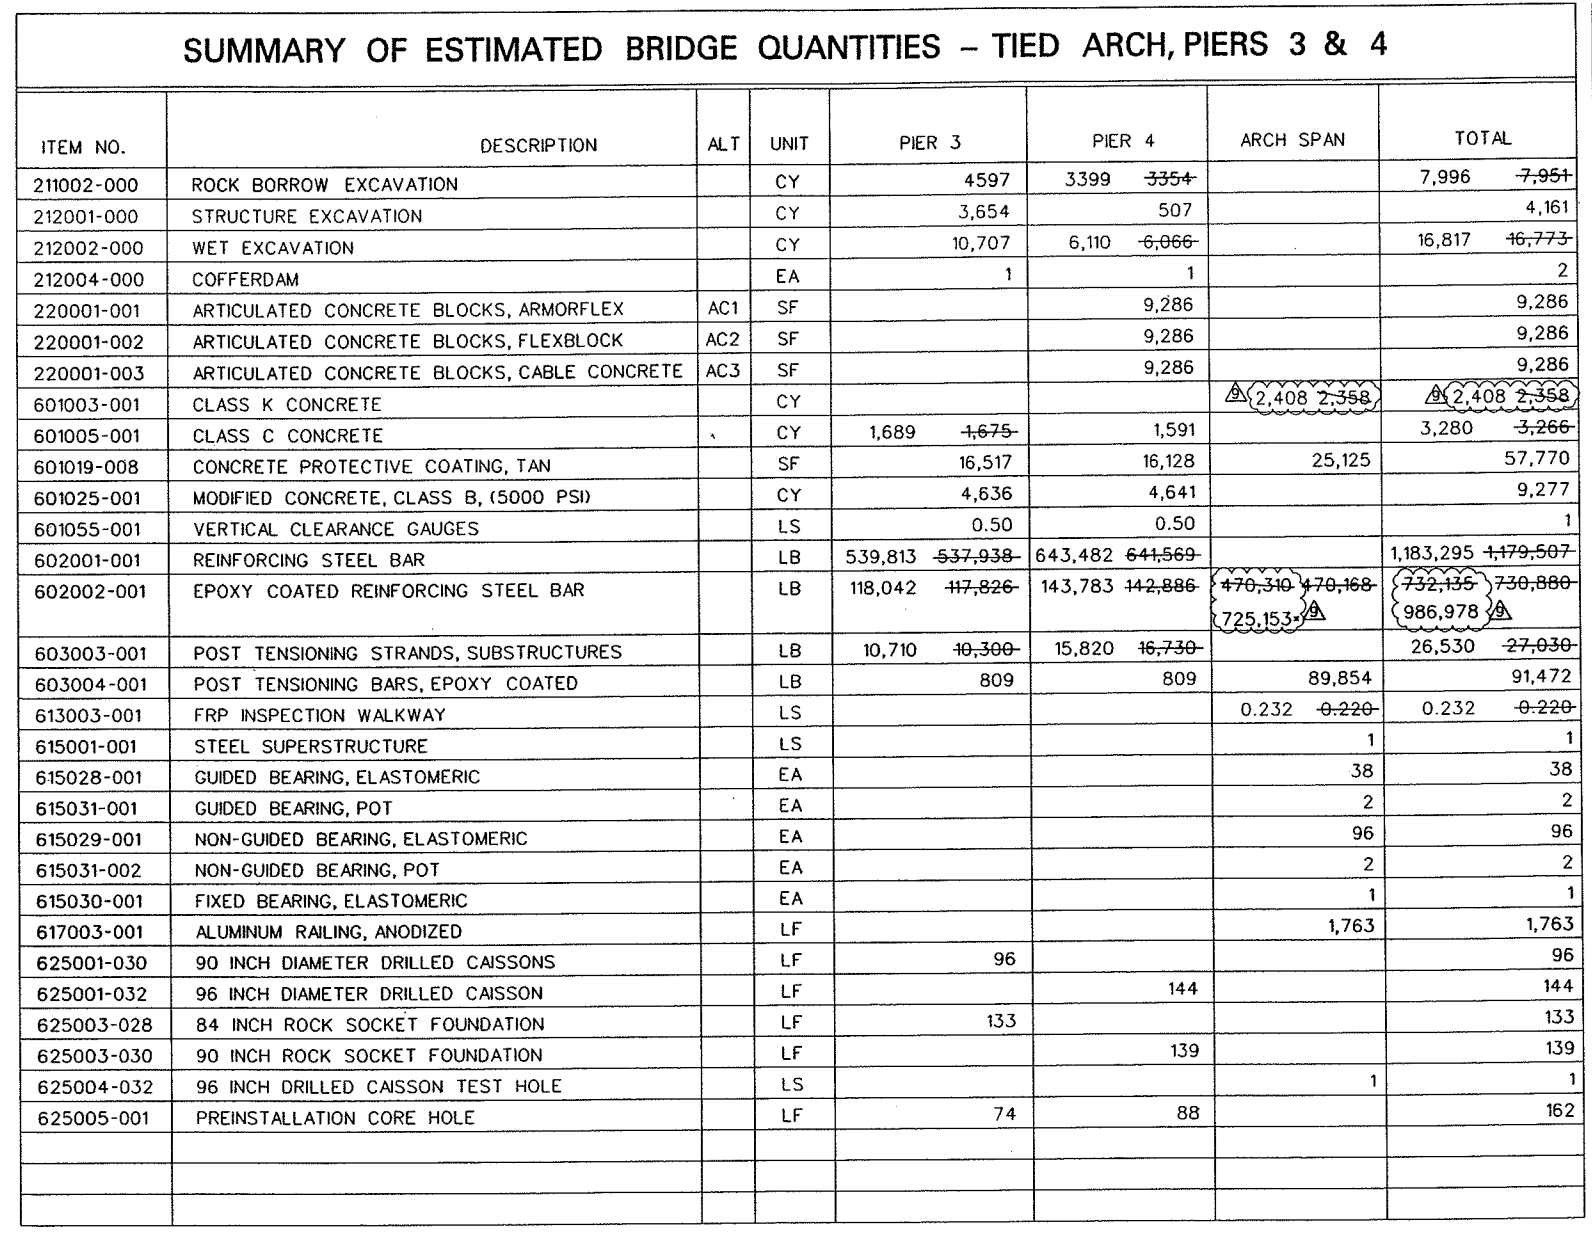
\includegraphics[trim={0 0 0 0},clip, width=0.6\textwidth]{overleaf/Appendix/Design drawings/estimated bridge quantities.PNG}
    \caption{Summary of estimated bridge quantities}
    \label{fig:bridge_quantities}
\end{figure}
\begin{figure}[H]
    \centering
    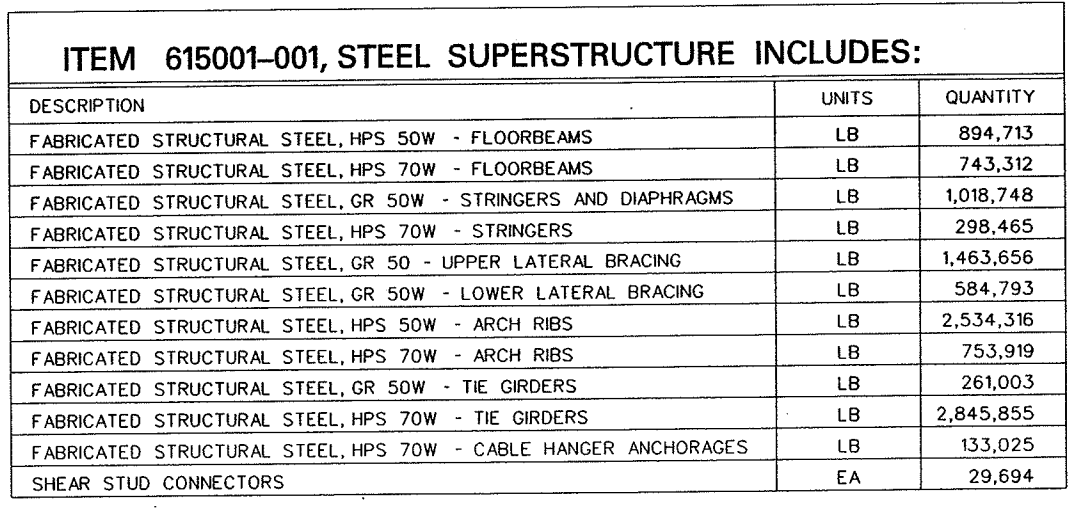
\includegraphics[trim={0 0 0 0},clip, width=0.6\textwidth]{overleaf/Appendix/Design drawings/Steel superstructure.PNG}
    \caption{Estimated steel quantities}
    \label{fig:steel_quantities}
\end{figure}

\begin{table}[H]
\centering
\begin{tabular}{lccc}
\hline
Component & Total weight & Length  & Distributed weight \\
          & {[}kN{]}     & {[}m{]} & {[}kN/m{]}         \\ \hline
Arch      & \SI{17524}{}        & 293.9   & 29.8               \\
Deck      & \SI{61776}{}        & 267.8   & 115.3              \\
Tie       & \SI{14116}{}        & 267.8   & 26.4               \\
Hangers   & \SI{401}{}          & \SI{1132}{}    & 0.35               \\
Utilities & \SI{9388}{}         & 267.8   & 35.1               \\
Total     & \SI{93817}{}        & 267.8   & 210.2              \\ \hline
\end{tabular}
\caption{Estimated weights of the components}
\label{tab:weights}
\end{table}

\subsection{Design verifications} \label{app:design_verifications}
The design verifications of the arch rib, the tie girder and the hangers are presented in Figs. \ref{fig:arch_design_verification} to \ref{fig:hanger_design_verification}.
\begin{figure}[H]
    \centering
    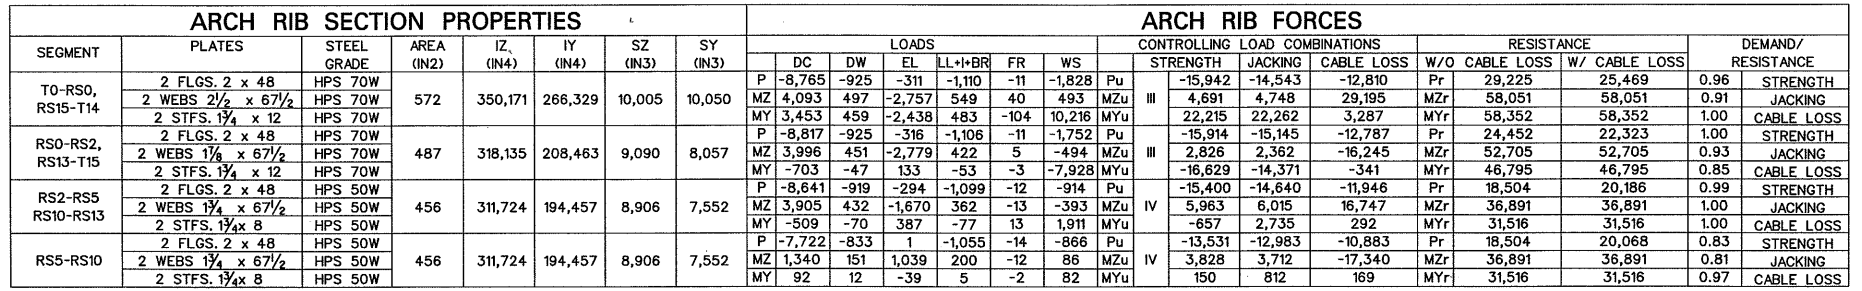
\includegraphics[width=\textwidth]{overleaf/Appendix/Design drawings/arch rib verifications.PNG}
    \caption{Design verifications of the arch rib segments}
    \label{fig:arch_design_verification}
\end{figure}
\begin{figure}[H]
    \centering
    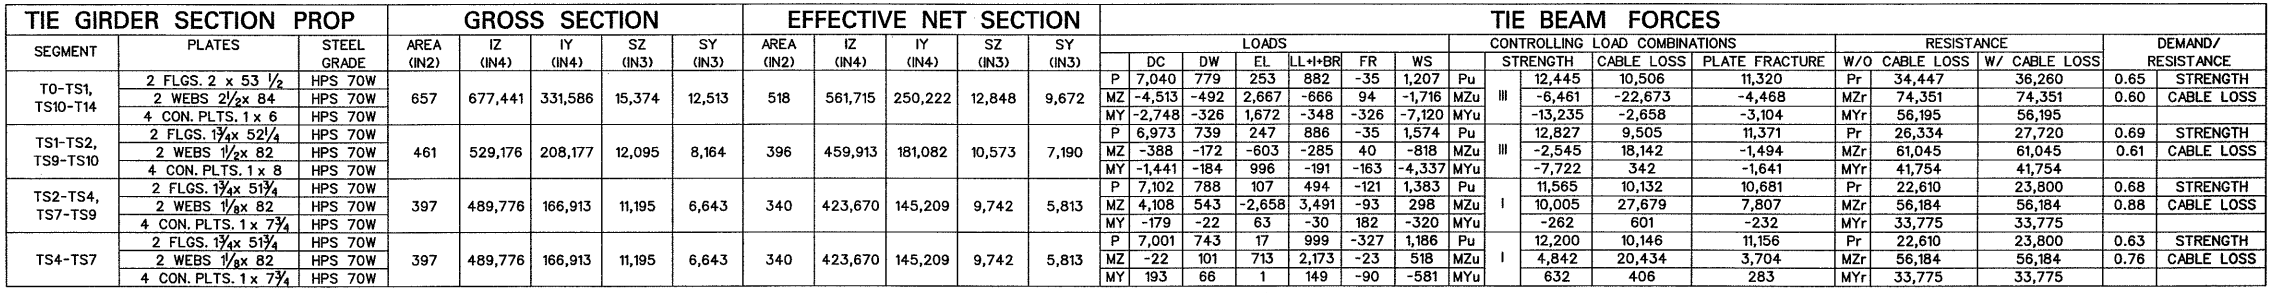
\includegraphics[width=\textwidth]{overleaf/Appendix/Design drawings/tie girder verifications.PNG}
    \caption{Design verifications of the tie girder segments}
    \label{fig:tie_design_verification}
\end{figure}
\begin{figure}[H]
    \centering
    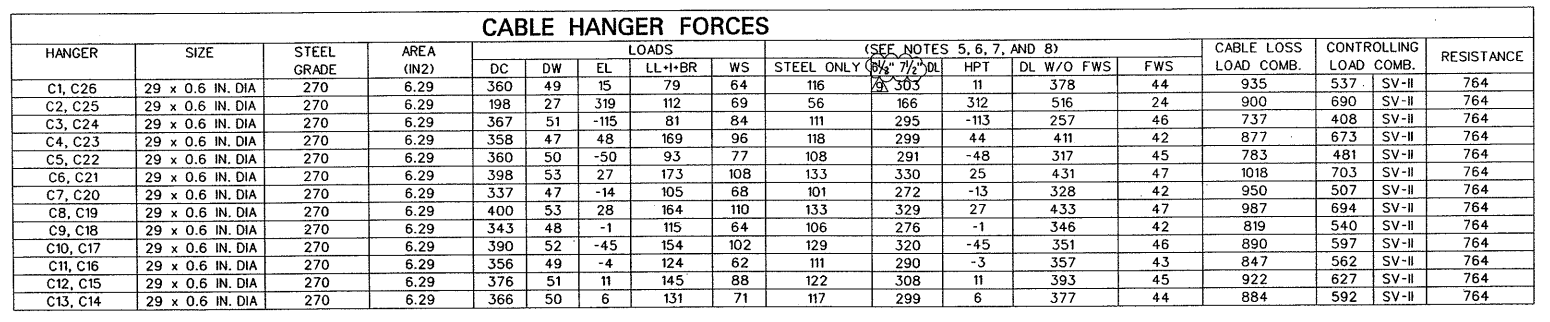
\includegraphics[width=\textwidth]{overleaf/Appendix/Design drawings/cable verifications.PNG}
    \caption{Design verifications of the hangers}
    \label{fig:hanger_design_verification}
\end{figure}



\newpage
\section{Model}
\label{AppendixModel}
\subsection{Hangers}
\label{Appendix_A_Hangers}
In this section, the non-linear effects of the hangers are considered. Assuming a parabolic displacement curve, the secondary effects are approximated by Eq. \eqref{eq:cable}, which gives the cable elongation $\delta$ at a stress of $\sigma_2$. Where $a$ is the horizontal component of the cable length $c$ at a stress of $\sigma_1$, $E$ is the modulus of elasticity and $\gamma$ is the weight of the cable \cite{NIELS}. 

\begin{equation}
    \frac{\delta}{c}= \frac{\sigma_2-\sigma_1}{E} 
    + \frac{\gamma^2\,c^2}{24}\,\left(\frac{1}{\sigma_1^2} -\frac{1}{\sigma_2^2} \right) 
    + \frac{\gamma^2\,c^2}{12\,E}\,\left(\frac{1}{\sigma_2} -\frac{1}{\sigma_1} \right)
    \label{eq:cable}
\end{equation}

To judge the influence on the Blennerhassett Island Bridge, the following values are assumed: $a=\SI{26}{m}$, $c=\SI{59.5}{m}$, $E=\SI{196}{GPa}$, $\gamma=\SI{78.5}{kN/m^3}$ and $\sigma_1=0.45\,f_y=\SI{750}{MPa}$. The elongation of the cable is compared to the assumed linear elastic behaviour of a rod, which is shown in Fig. \ref{fig:hanger_approximation}.

\begin{figure}[H]
    \centering
    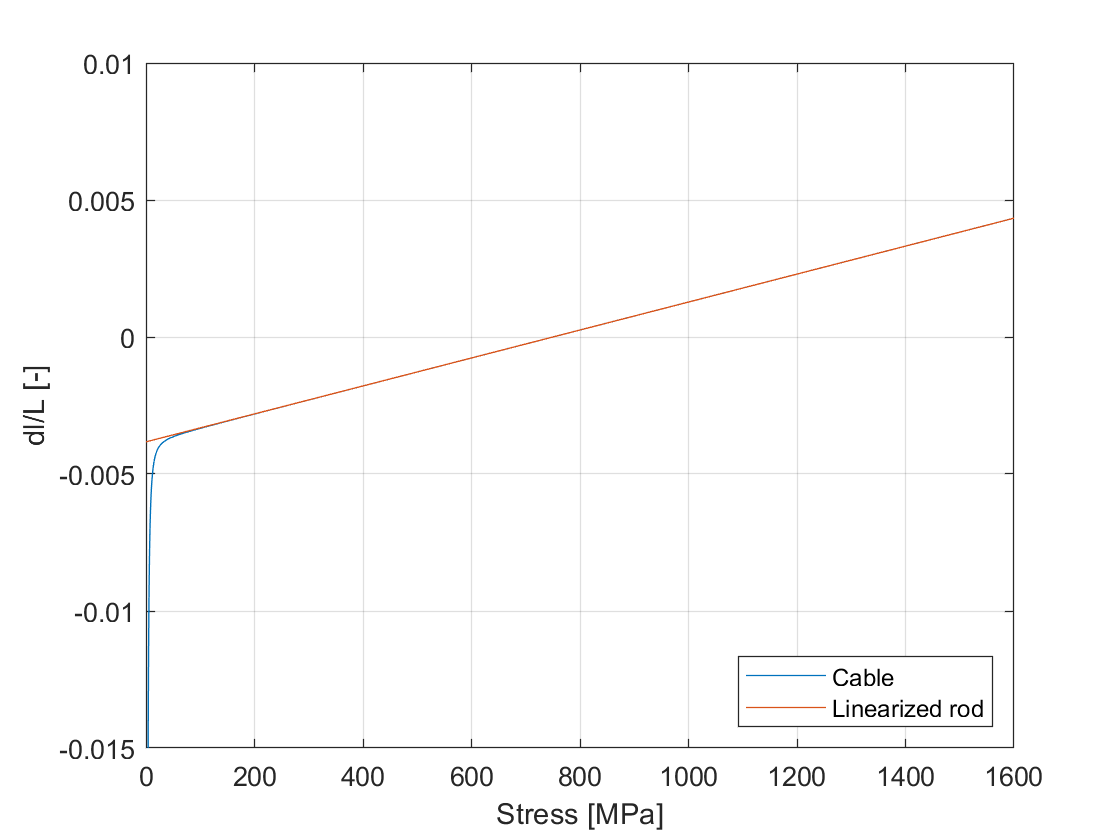
\includegraphics[width=0.7\textwidth]{overleaf/Appendix/Pictures/hanger_approximation.png}
    \caption{Cable elongation considering secondary effects}
    \label{fig:hanger_approximation}
\end{figure}

Only for cables stresses below \SI{100}{MPa}, which corresponds to 6\% of its yield stress, secondary effects become relevant. As stresses in this range are not occurring in any calculation, secondary effects can be neglected.

\newpage
\subsection{Live loading} \label{Appendix_Liveloading}
In this section, the arrangement of the live loads on the deck is investigated. The three design states strength, cable replacement and cable loss are treated individually as different circumstances apply. The live load relevant for fatigue can then be derived from the strength limit state. In the first step, the location of each lane is defined. According to the AASHTO design provisions, the width of every lane is equal to $\SI{12}{ft} = \SI{3.7}{m}$ of which \SI{3}{m} are loaded and the center of the applied forces $x_c$ can be derived \cite{AASHTO}. The force applied to the tie girder $F_r$ can then be calculated according to Eq. \ref{eq:reaction} using the width of the deck $w_{deck}=\SI{107}{ft}=\SI{32.6}{m}$.
\begin{equation}
    F_r = \frac{x_c}{w_{deck}}
    \label{eq:reaction}
\end{equation}
In a second step, the amount of loaded lanes under the consideration of the multiple presence factor (MPF) is determined. As the multiple presence factor decreases with the number of loaded lanes, each possibility is calculated to find the worst arrangement. The calculations are conducted for a unit lane load. The obtained factor relates the load on each lane to the load applied to the investigated tie girder. The factor can then be used for the calculation of the force on the tie of the distributed lane load ($q_{LL}=\SI{9.3}{kN/m}$) as well as of the design truck load ($Q_{LL}=\SI{325}{kN}$). For the design truck load, an additional dynamic multiplier of 1.33 is taken into account. 

\subsubsection*{Vehicular use} \label{Appendx_A_Live_loading_1}
In the first strength limit state, the entire width of the deck is available to traffic. The lanes are arranged as densely to one side as possible with the first lane starting at $\SI{4.6}{ft}=\SI{1.4}{m}$ from the investigated arch plane. The calculations presented in Table \ref{tab:app_ll_uls} show that the worst arrangement results with six loaded lanes. 

\begin{table}[H]
\centering
\begin{tabular}{cccccccccccc}
\cline{2-11}
             & Lane     &  & 1    & 2    & 3    & 4    & 5    & 6    & 7    & 8    &      \\
             & Centroid &  & 2.9  & 6.6  & 10.2 & 13.9 & 17.5 & 21.2 & 24.8 & 28.5 &      \\
             & Reaction &  & 0.91 & 0.80 & 0.69 & 0.57 & 0.46 & 0.35 & 0.24 & 0.13 &      \\ \hline
Loaded Lanes & MPF      &  &      &      &      &      &      &      &      &      & Sum  \\ \hline
1            & 1.2      &  & 1.09 &      &      &      &      &      &      &      & 1.09 \\
2            & 1.0      &  & 0.91 & 0.80 &      &      &      &      &      &      & 1.71 \\
3            & 0.85     &  & 0.77 & 0.68 & 0.58 &      &      &      &      &      & 2.04 \\
4            & 0.75     &  & 0.68 & 0.60 & 0.52 & 0.43 &      &      &      &      & 2.23 \\
5            & 0.70     &  & 0.64 & 0.56 & 0.48 & 0.40 & 0.32 &      &      &      & 2.40 \\
6            & 0.65     &  & 0.59 & 0.52 & 0.45 & 0.37 & 0.30 & 0.23 &      &      & 2.46 \\
7            & 0.60     &  & 0.55 & 0.48 & 0.41 & 0.34 & 0.28 & 0.21 & 0.14 &      & 2.41 \\
8            & 0.55     &  & 0.50 & 0.44 & 0.38 & 0.32 & 0.25 & 0.19 & 0.13 & 0.07 & 2.28 \\ \hline
\end{tabular}
\caption{Force on tie girder for ultimate limit state under unit lane load}
\label{tab:app_ll_uls}
\end{table}

Six loaded lanes yield a factor of 2.46. Hence the load applied on the investigated arch plane can be calculated according to Eqs. \eqref{eq:q_ll_uls} and \eqref{eq:Q_ll_uls}. The decisive arrangement is illustrated in Fig. \ref{fig:app_hangers_uls}.
\begin{equation}
    q_{ll, uls} = 2.46 \cdot \SI{9.3}{kN/m} = \SI{22.9}{kN/m}
    \label{eq:q_ll_uls}
\end{equation}
\begin{equation}
    Q_{ll, uls} = 2.46 \cdot 1.33 \cdot \SI{325}{kN} = \SI{1063}{kN}
    \label{eq:Q_ll_uls}
\end{equation}

\begin{figure}[H]
    \centering
    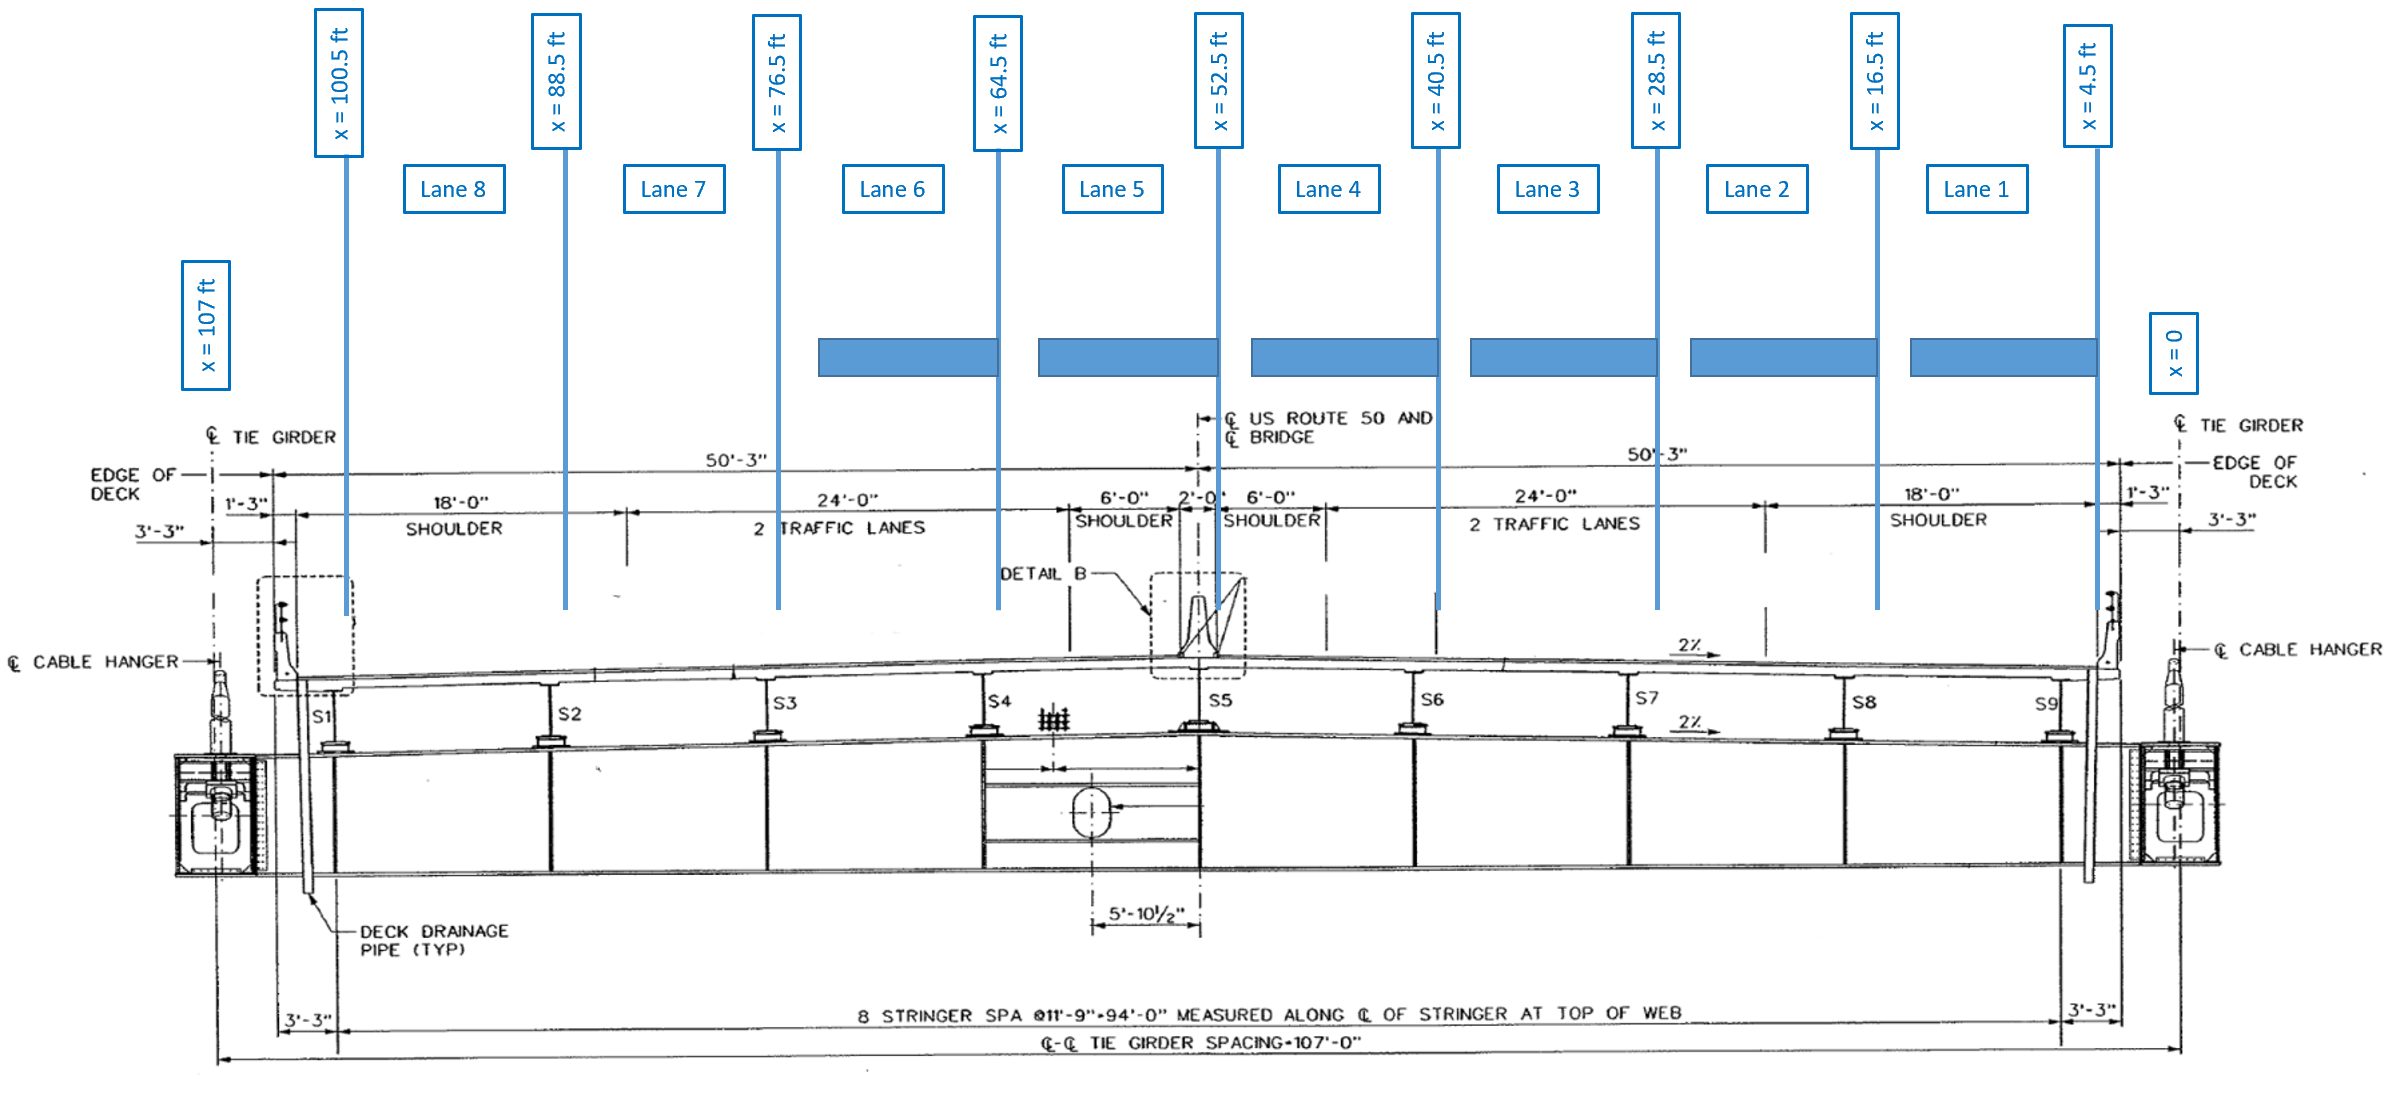
\includegraphics[width=\textwidth]{overleaf/Appendix/Pictures/Cross_Section_LL_ULS.PNG}
    \caption{Live load arrangement in the strength limit state}
    \label{fig:app_hangers_uls}
\end{figure}


\subsubsection*{Fatigue} \label{Appendx_A_Live_loading_15}
The fatigue limit state is investigated according to the recommendations for stay cable design, testing and installation by the Post Tensioning Institute (PTI). The corresponding loading is composed of a single design truck which occupies the lane resulting in the highest effect on the investigated stay cable \cite{PTI}. It corresponds to the lane closest to the border in this case, for which, according to Table \ref{tab:app_ll_uls}, the force on the tie girder is equal to 91\% of the design truck load. It results in the fatigue load according to Eq. \ref{eq:Q_fat}.

\begin{equation}
    Q_{fat} = 0.91 \cdot \SI{325}{kN} = \SI{296}{kN}
    \label{eq:Q_fat}
\end{equation}

\subsubsection*{Cable replacement} \label{Appendx_A_Live_loading_2}
In the event of cable replacement, one lane is shifted away from the hanger being exchanged. Besides that, the lanes are located at the same positions as in the ultimate limit state. A load for the replacement truck is disregarded for in this investigation. The calculation of the different arrangements is presented in Table \ref{tab:app_ll_hanger_replacement}.
\begin{table}[H]
\centering
\caption{Force on tie girder for hanger replacement under unit lane load}
\label{tab:app_ll_hanger_replacement}
\resizebox{.8\textwidth}{!}{%
\begin{tabular}{cccccccccccc}
\cline{2-11}
             & Lane     &  & 1    & 2    & 3    & 4    & 5    & 6    & 7    & 8    &      \\
             & Centroid &  & 2.9  & 6.6  & 10.2 & 13.9 & 17.5 & 21.2 & 24.8 & 28.5 &      \\
             & Reaction &  & 0.91 & 0.80 & 0.69 & 0.57 & 0.46 & 0.35 & 0.24 & 0.13 &      \\ \hline
Loaded Lanes & MPF      &  &      &      &      &      &      &      &      &      & Sum  \\ \hline
1            & 1.2      &  & -    & 0.96 &      &      &      &      &      &      & 0.96 \\
2            & 1.0      &  & -    & 0.80 & 0.69 &      &      &      &      &      & 1.49 \\
3            & 0.85     &  & -    & 0.68 & 0.58 & 0.49 &      &      &      &      & 1.75 \\
4            & 0.75     &  & -    & 0.60 & 0.52 & 0.43 & 0.35 &      &      &      & 1.89 \\
5            & 0.70     &  & -    & 0.56 & 0.48 & 0.40 & 0.32 & 0.25 &      &      & 2.01 \\
6            & 0.65     &  & -    & 0.52 & 0.45 & 0.37 & 0.30 & 0.23 & 0.15 &      & 2.02 \\
7            & 0.60     &  & -    & 0.48 & 0.41 & 0.34 & 0.28 & 0.21 & 0.14 & 0.08 & 1.94 \\ \hline
\end{tabular}
}
\end{table}

The resulting loads on the investigated arch plane are presented in Eqs. \eqref{eq:q_ll_repl} and \eqref{eq:Q_ll_repl}.
\begin{equation}
    q_{ll, repl} = 2.02 \cdot \SI{9.3}{kN/m} = \SI{18.8}{kN/m}
    \label{eq:q_ll_repl}
\end{equation}
\begin{equation}
    Q_{ll, repl} = 2.02 \cdot 1.33 \cdot \SI{325}{kN} = \SI{874}{kN}
    \label{eq:Q_ll_repl}
\end{equation}

\subsubsection*{Cable loss} \label{Appendx_A_Live_loading_3}
In the extreme event of cable loss, not the deck's entire width is available to the live loads. For this case, only the four actual marked lanes are available. Their locations were taken from the design drawings. The investigation in Table \ref{tab:app_ll_cable_loss} shows that all of these lanes are loaded in the worst arrangement.
\begin{table}[H]
\centering
\caption{Force on tie girder for cable loss under unit lane load}
\label{tab:app_ll_cable_loss}
\begin{tabular}{cccccccc}
\cline{2-7}
             & Lane     &  & 1    & 2    & 3    & 4    &      \\
             & Centroid &  & 8.4  & 12.0 & 20.0 & 23.6 &      \\
             & Reaction &  & 0.74 & 0.63 & 0.39 & 0.28 &      \\ \hline
Loaded Lanes & MPF      &  &      &      &      &      & Sum  \\ \hline
1            & 1.2      &  & 0.89 &      &      &      & 0.89 \\
2            & 1.0      &  & 0.74 & 0.63 &      &      & 1.37 \\
3            & 0.85     &  & 0.63 & 0.54 & 0.33 &      & 1.50 \\
4            & 0.75     &  & 0.56 & 0.47 & 0.29 & 0.21 & 1.53 \\ \hline
\end{tabular}
\end{table}

The loads resulting on the tie girder are calculated in Eqs. \eqref{eq:q_ll_loss} and \eqref{eq:Q_ll_loss}.
\begin{equation}
    q_{ll, loss} = 1.53 \cdot \SI{9.3}{kN/m} = \SI{14.2}{kN/m}
    \label{eq:q_ll_loss}
\end{equation}
\begin{equation}
    Q_{ll, loss} = 1.42 \cdot 1.33 \cdot \SI{325}{kN} = \SI{660}{kN}
    \label{eq:Q_ll_loss}
\end{equation}

An illustration of the load arrangement for the event of cable loss is presented in Fig. \ref{fig:app_hangers_cable_loss}.

\begin{figure}[H]
    \centering
    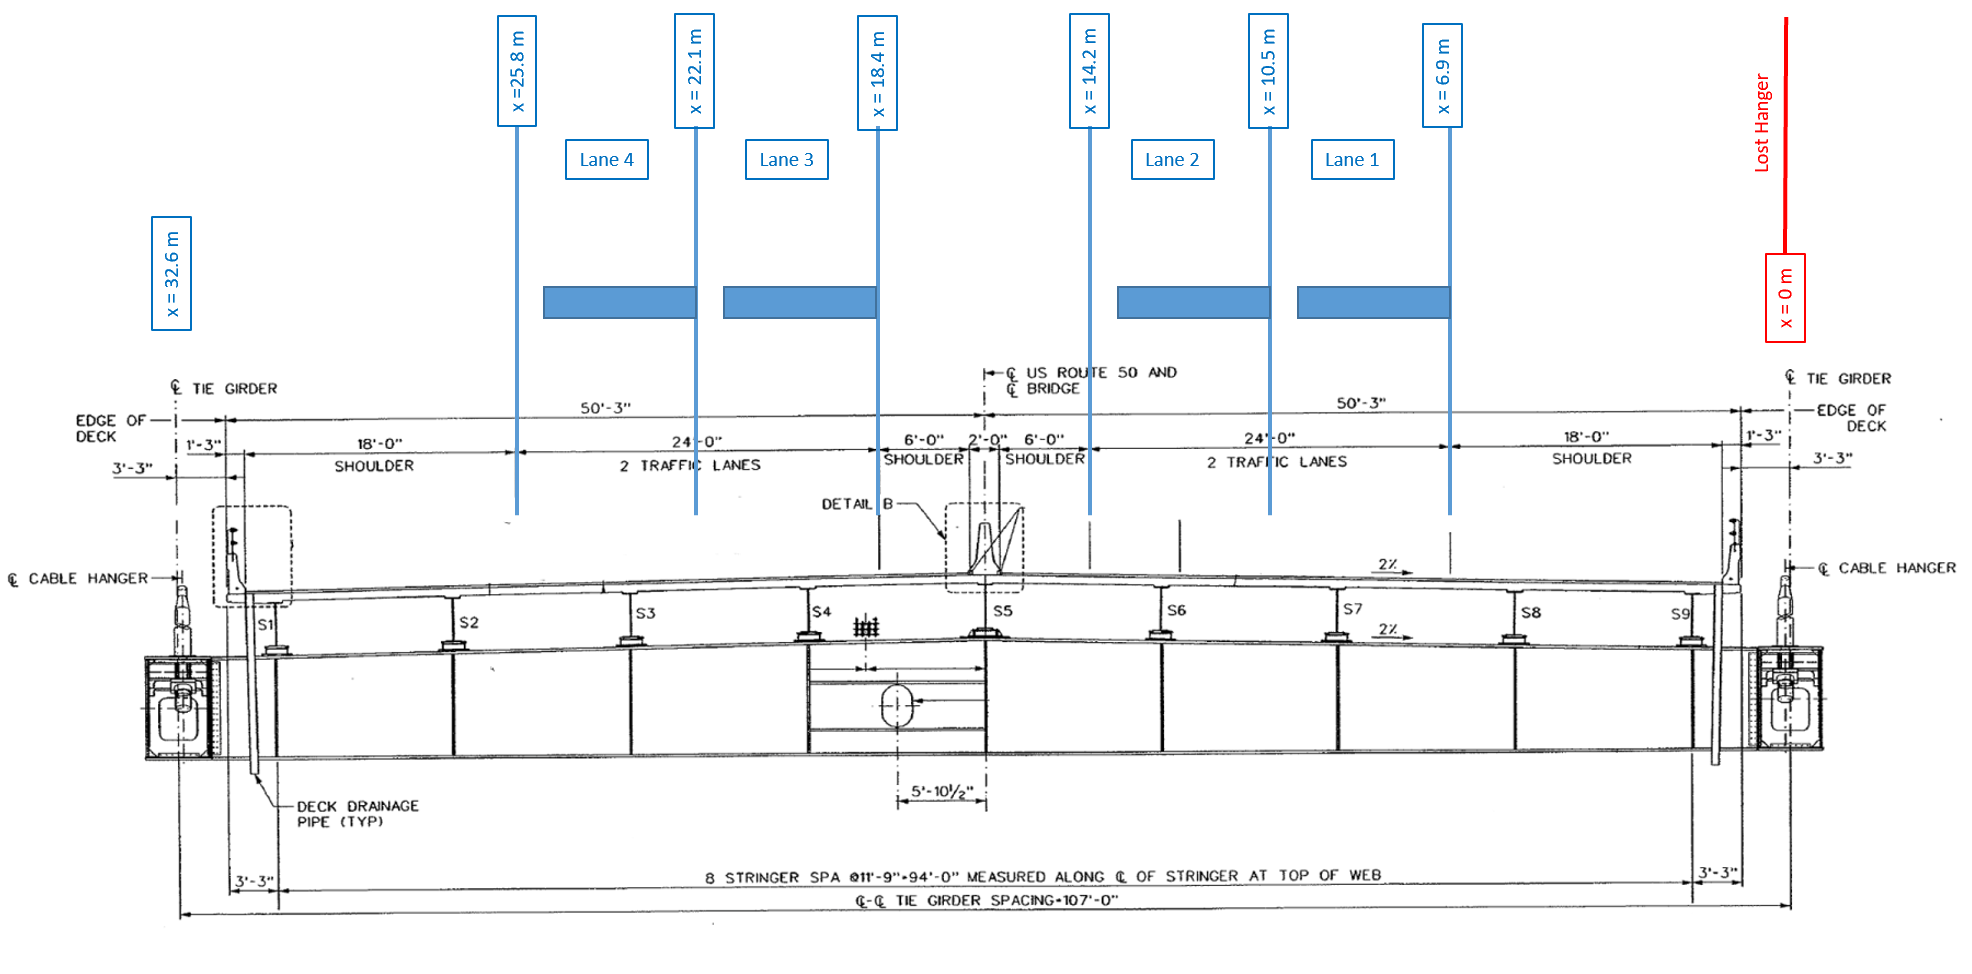
\includegraphics[width=\textwidth]{overleaf/Appendix/Pictures/Cross_Section_LL_Cable Loss.PNG}
    \caption{Live load arrangement for cable loss}
    \label{fig:app_hangers_cable_loss}
\end{figure}

\newpage
\subsection{Verification}

\newpage
\section{Optimisation methods}
In this chapter, the mathematical background of the used optimisation methods is briefly explained. First, the methods related to the assignment of the permanent hanger forces are introduced in Sec. \ref{app:moment_min} and \ref{app:lsq}. The calculation of the thrust line, including the self weight of the arch, is explained in Sec. \ref{app:thrust_line}.

\subsection{Absolute moment minimisation} \label{app:moment_min}
In a n-times statically indeterminate structure, there are n supernumerary forces or moments. These forces are present in the initial configuration even without any applied loads. The elastic answer of the structure for the different load cases is simply added to obtain the respective effects. It is the goal of an efficient initial configuration to simplify the design verifications by counteracting the effects expected in the various load cases. Here, this is achieved by minimising the permanent moment distribution in the tie and potentially the arch as well. The permanent moment distribution at m points along the considerded component $M \in \mathbb{R}^m$ can be described by Eq. \eqref{eq:perm_mom}. 
\begin{equation}
    {\bf M} = {\bf M_0} + \sum_{i=1}^{n} {\bf M_i} \cdot X_i = {\bf M_0} + {\bf M_{sn}} \cdot {\bf X}
    \label{eq:perm_mom}
\end{equation}
where ${\bf M_0} \in \mathbb{R}^m$ is the moment distribution of the permanent loads on the basic system, ${\bf M_i} \in \mathbb{R}^m$ is the moment distribution of the i-th supernumerary unit force, ${X_i} \in \mathbb{R}$ is the i-th supernumerary force. The later two can be combined into the matrix of supernumerary moments ${\bf M_{sn}} \in  \mathbb{R}^{m\times n}$ and the vector of supernumerary forces or moments ${\bf X} \in \mathbb{R}^n$.

\begin{figure}[H]
\centering
\begin{subfigure}{0.5\textwidth}
    \centering
    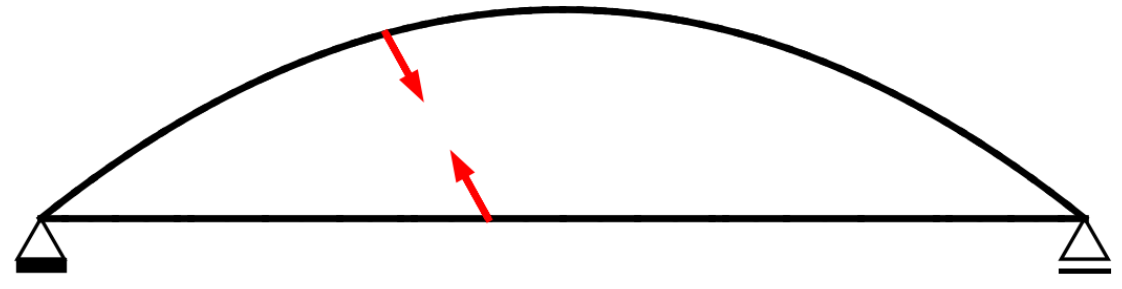
\includegraphics[trim={0 0cm 0 0},clip, width=0.9\textwidth]{overleaf/Appendix/Pictures/min_1.PNG}
    \caption{Basic system and supernumerary force}
    \label{fig:Minimisation_1}
\end{subfigure}%
\begin{subfigure}{.5\textwidth}
    \centering
    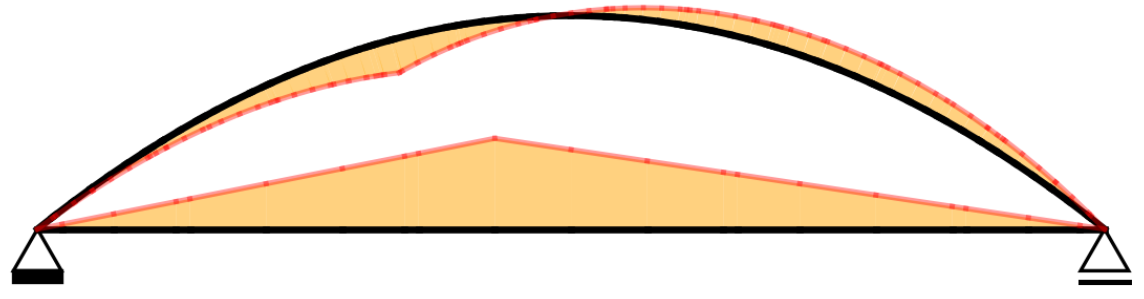
\includegraphics[trim={0 0cm 0 0},clip, width=0.9\textwidth]{overleaf/Appendix/Pictures/min_2.PNG}
    \caption{Moments under supernumerary force}
    \label{fig:Minimisation_2}
\end{subfigure}
\caption{Moment distribution of supernumerary force}
\label{fig:Minimisation}
\end{figure}

The problem of minimising the absolute maximum moments can be formulated according to Eq. \eqref{eq:minimisation}, where the absolute maximum moment is expressed as the infinity norm.
\begin{align}
    \underset{{\bf X}}{\text{Minimize}} \quad & f({\bf X}) = \max({\bf M}, -{\bf M}) = \|{\bf M_0} + {\bf M_{sn}} \cdot {\bf X}\|_{\infty} 
    \label{eq:minimisation}
\end{align}

The helper variable $t$ is introduced, which describes the moment magnitude which is larger than the absolute moments in ${\bf M}$. With the help of $t$, the previously stated problem can be formulated as a linear programming problem, as shown in Eq. \eqref{eq:minimisation_2}.
\begin{align}
    \underset{t, {\bf X}}{\text{Minimize}} \quad & f(t) = t \label{eq:minimisation_2} \\
    \text{s.t.} \quad & {\bf M_0} + {\bf M_{sn}} \cdot {\bf X} - t {\bf 1} \leq  0 \nonumber \\
    \quad & {-\bf M_0} - {\bf M_{sn}} \cdot {\bf X} - t {\bf 1} \leq 0 \nonumber
\end{align}

Additionally, bounds for the permanent hanger forces can be specified as further inequality conditions. It should be noted that under the consideration of symmetry the amount of variables in the linear problem can be reduced. If only the moment distribution in the tie is optimised, it makes sense to only consider vertical forces at each hanger node. In a second step, the optimised vertical forces are assigned to the two hangers at the node.

\subsection{Least squares moments} \label{app:lsq}
As an alternative approach, the supernumerary forces can be determined using the method of least squares. The objective of this method is to find supernumerary forces which counteract a certain moment distribution, for example the moment distribution on the basic system. Using the variables which were introduced in the previous section, the objective is described by Eq. \eqref{eq:lsq_1}.
\begin{equation}
    {\bf M_{sn}} \cdot {\bf X} = -{\bf M_0}
    \label{eq:lsq_1}
\end{equation}
As this yields an overdetermined system, the equations cannot be solved simultaneously. Using the method of least squares, the sum of the squared deviations can be minimised by solving the determined system in Eq. \eqref{eq:lsq_2}.
\begin{equation}
    ({\bf M_{sn}}^T\,{\bf M_{sn}}) \cdot {\bf X} = -{\bf M_{sn}}^T\,{\bf M_0}
    \label{eq:lsq_2}
\end{equation}
The drawback of this method is that no bounds for the hanger forces can be specified. However, this method is particularly useful, if the hanger forces have been optimised by minimising the moments on the tie girder. At this point, the permanent tension force in the tie girder is still undefined, as it does not affect the moment distribution. It can then be calculated by considering the moment distribution in the arch rib, minimising the squares of its moment distribution. In this case, the approach is fast and can even be solved without using linear algebra as there is only one variable.

\subsection{Thrust line derivation} \label{app:thrust_line}
There are two thrust line derivations relevant for this Thesis. In Section \ref{app:continuous}, the thrust line is derived for the hypothetical case of an infinitely dense hanger arrangement. For a discrete hanger arrangement the thrust line can be derived according to the method described in Section \ref{app:discrete}. Both methods take the weight of the arch into account.

\subsubsection{Continuous hanger arrangement}\label{app:continuous}
In a first step, the hanger force densities of each hanger set are determined without the consideration of the arch. There are multiple possibilities to do so. For example, they could be calculated to be in equilibrium with the permanent vertical force $q$, depending on their angles of inclination $\alpha$ and $\beta$. However, horizontal equilibrium is an unnecessary condition, as the tie is affected by significant tension forces anyway. Therefore, it is proposed to assign force densities of identical magnitude to hangers on each infinitesimal element, as illustrated in Fig. \ref{fig:continuous_1}. Also the resultant forces $F_L$ and $F_R$ are shown.
\begin{figure}[H]
    \centering
    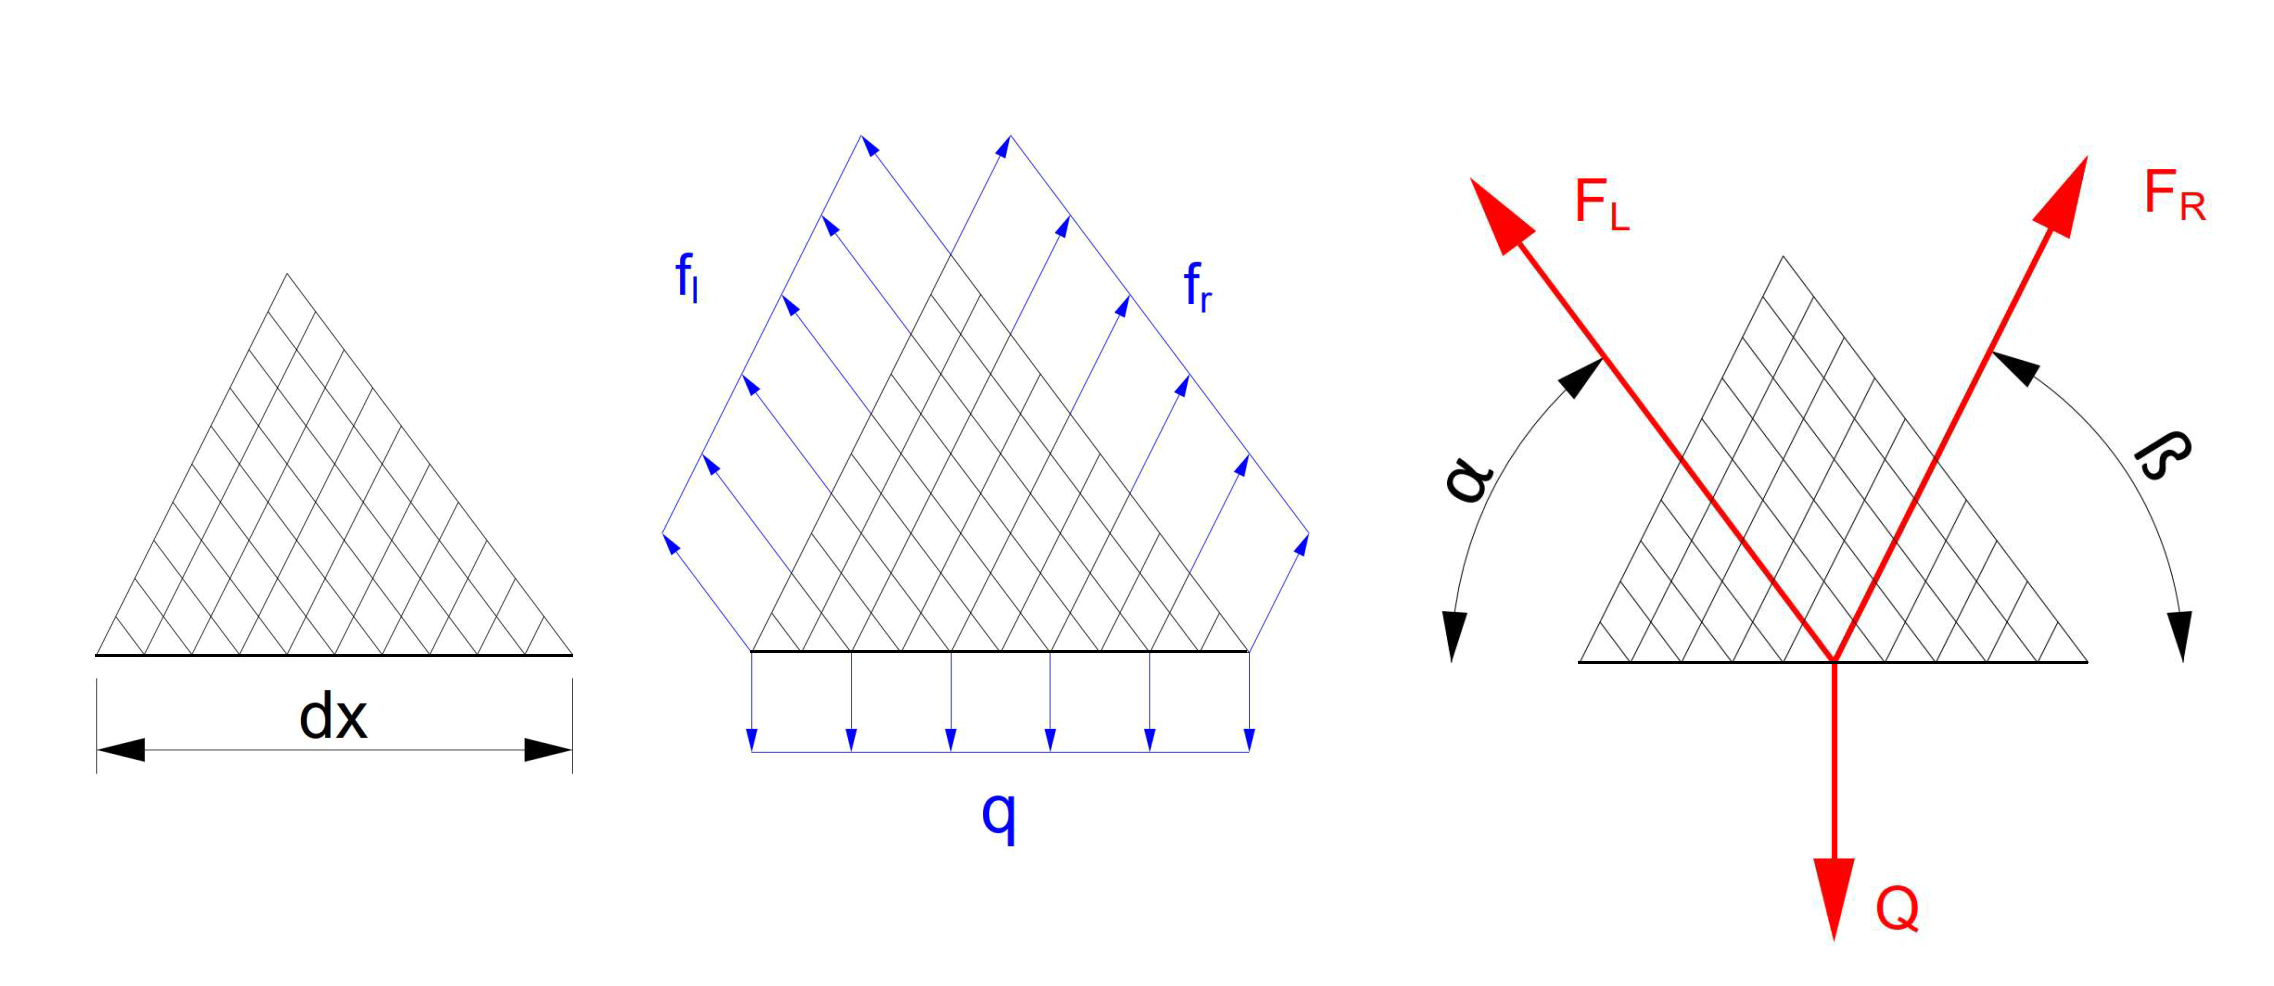
\includegraphics[width=0.8\textwidth]{overleaf/Appendix/Pictures/continuous_thrust_line_1.PNG}
    \caption{Hanger force densitites on an infinitesimal element}
    \label{fig:continuous_1}
\end{figure}

The corresponding hanger force densities $f_l$ and $f_r$ can be calculated according to Eq. \eqref{eq:continuous_1}.
\begin{equation}
    f_l=f_r=\frac{q}{\sin{\alpha}+ \sin{\beta}}
    \label{eq:continuous_1}
\end{equation}

While the thrust line can be described analytically by a differential equation, it is impossible to get an analytical solution for general hanger arrangement patterns. Therefore, the thrust line of the infinitesimal hanger arrangement is calculated in fixed horizontal steps of $dx$ starting from the crown, where a normal force $N_{crown}$ is assumed. If the step $dx$ is small, it can be assumed, that the inclination of the thrust line undergoes small changes in every step. At the beginning of each step the normal force $N_1$ is known, which also corresponds to the inclination of the thrust line. In each step, the change of height of the thrust line $dy$ is determined iteratively. It underlies the condition that the new inclination coincides with the inclination of the new normal force, which can be described by Eq. \ref{eq:continuous_2}.
\begin{equation}
    dy = \frac{dx}{2} \cdot \left(\frac{N_{1,y}}{N_{1,x}} + \frac{N_{2,y}}{N_{2,x}} \right)
    \label{eq:continuous_2}
\end{equation}

The new normal force $N_2$ is determined from force equilibrium considering the hanger forces and the self weight, both of which depend on $dy$. The self weight is determined from the length of the segment multiplied by the weight per meter. For the hanger forces, the lengths of the two hanger sets on the tie $dl_1$ and $dl_2$ affecting the considered arch segment are determined over geometrical considerations. Using the previously determined hanger force densities the resulting hanger force is determined. The calculation of a single step is illustrated in Fig. \ref{fig:continuous_2}.
\begin{figure}[H]
    \centering
    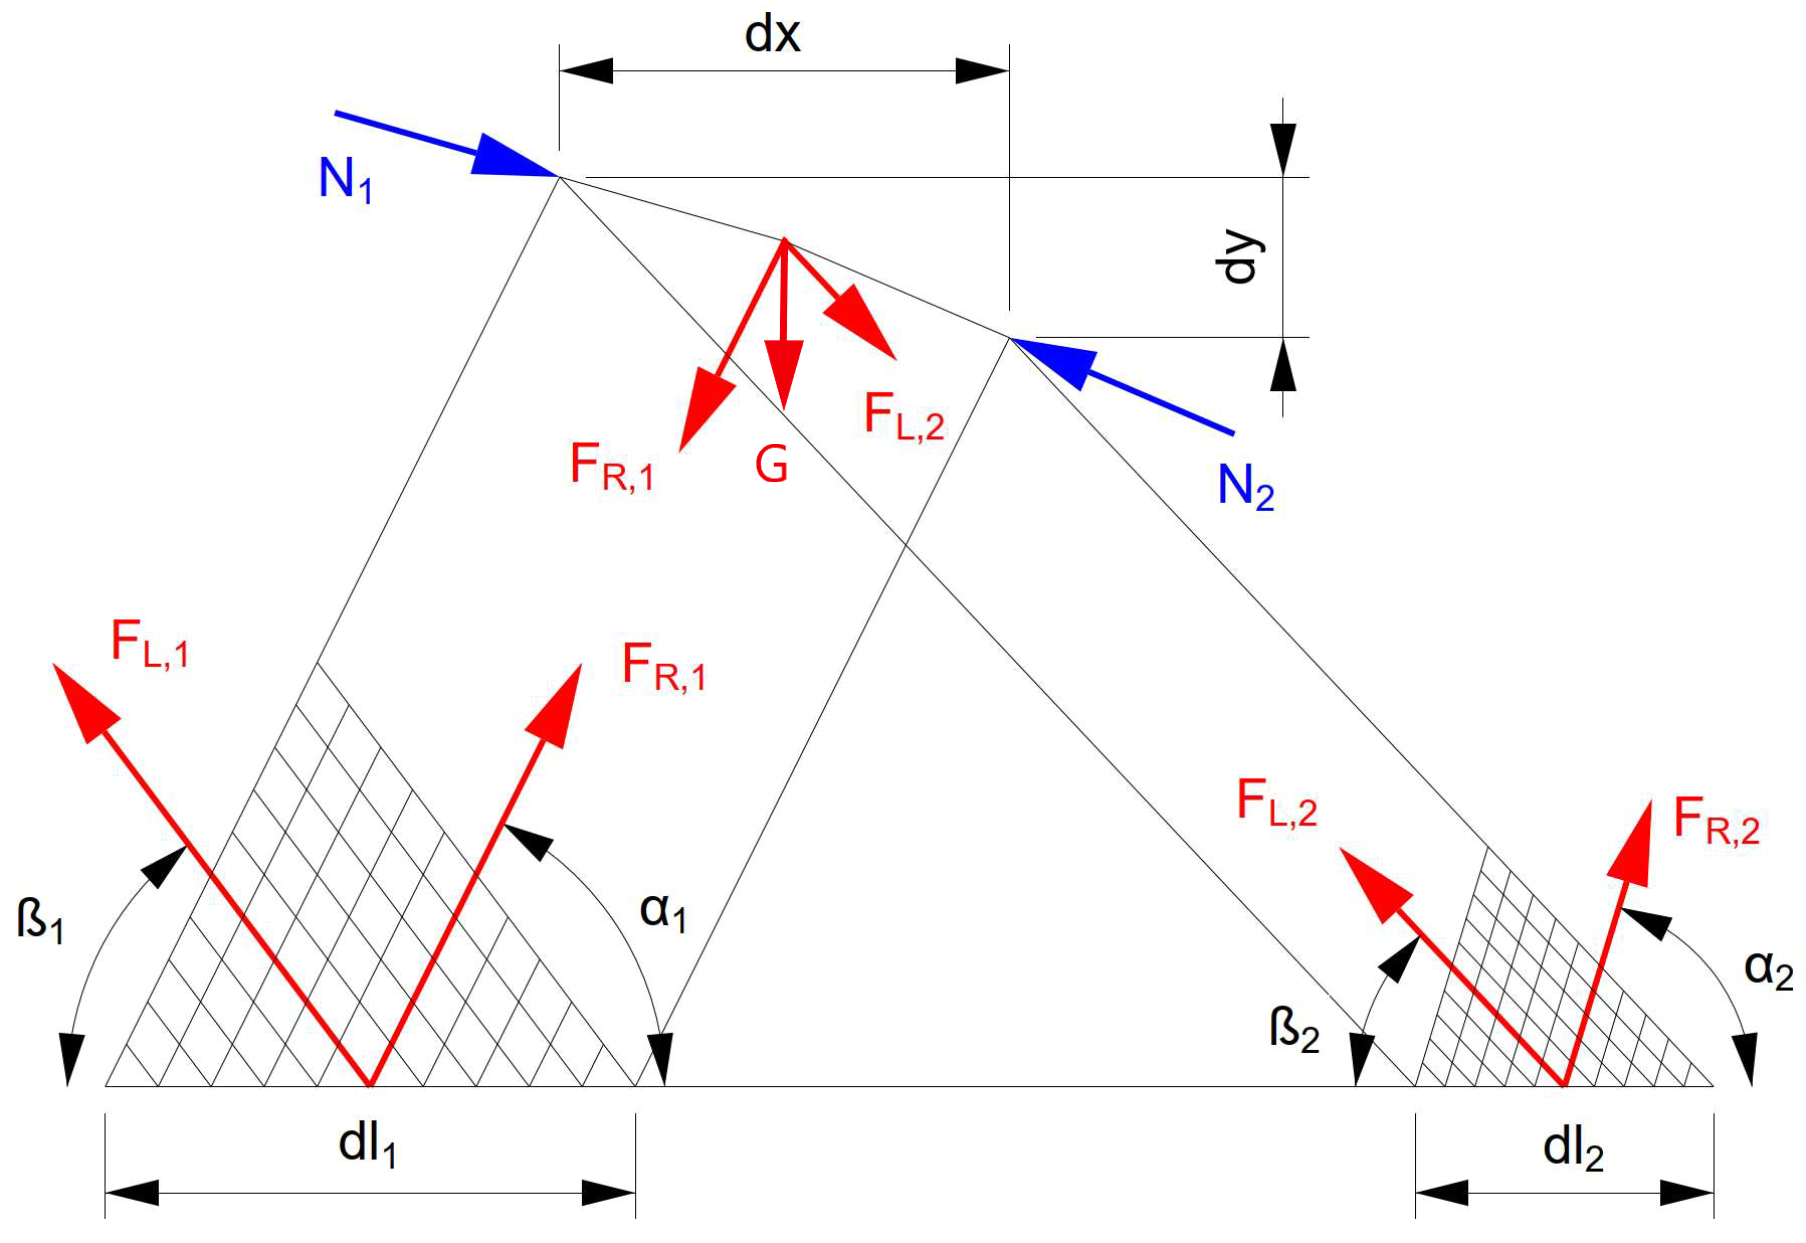
\includegraphics[width=0.8\textwidth]{overleaf/Appendix/Pictures/continuous_thrust_line.PNG}
    \caption{Derivation of the arch thrust line for a continuous hanger arrangement}
    \label{fig:continuous_2}
\end{figure}

Ultimately, the normal force in the crown $N_{crown}$ is determined iteratively for the thrust line to intersect the knuckle point. However, this normal force in the crown could also be determined from static considerations involving global longitudinal moment and the hanger force densities without the need of an iteration.


\subsubsection{Discrete hanger arrangement}\label{app:discrete}

Calculating the thrust line of a discrete hanger arrangement is a particular challenge as it is not known in which order the hangers intersect the thrust line beforehand. Therefore it is also calculated in steps. Similar to the continuous calculation, it is started from the crown with an estimated normal force $N_{crown}$ and the inclination at the beginning of every step corresponds to the ratio of the normal force components. Further, the arch's weight per horizontal meter is estimated from Eq. \ref{eq:g_arch}.

\begin{equation}
    g_{arch,x} = g_{arch} \cdot \sqrt{1+y'^2} = g_{arch} \cdot \sqrt{1+\left( \frac{N_{y}}{N_{x}} \right)^2}
    \label{eq:g_arch}
\end{equation}

Using this weight per horizontal meter, the parabolic thrust line can be estimated according to Eq. \ref{eq:discrete}. The height at the beginning of the current step is given by $y_1$ The second term gives the inclination of the normal force, which would continue the thrust line under no additional loading. The weight of the arch causes a slight curvature according to the third quadratic term.

\begin{equation}
    y(x) = y_1 - \frac{N_y}{N_x} \cdot x - \frac{g_{arch,x}}{2\cdot N_x}\cdot x^2
    \label{eq:discrete}
\end{equation}

Unless a hanger intersects the thrust line within the current step, the thrust line is continued by the step length $dx$. An illustration is given in Fig. \ref{fig:discrete_1}.

\begin{figure}[H]
    \centering
    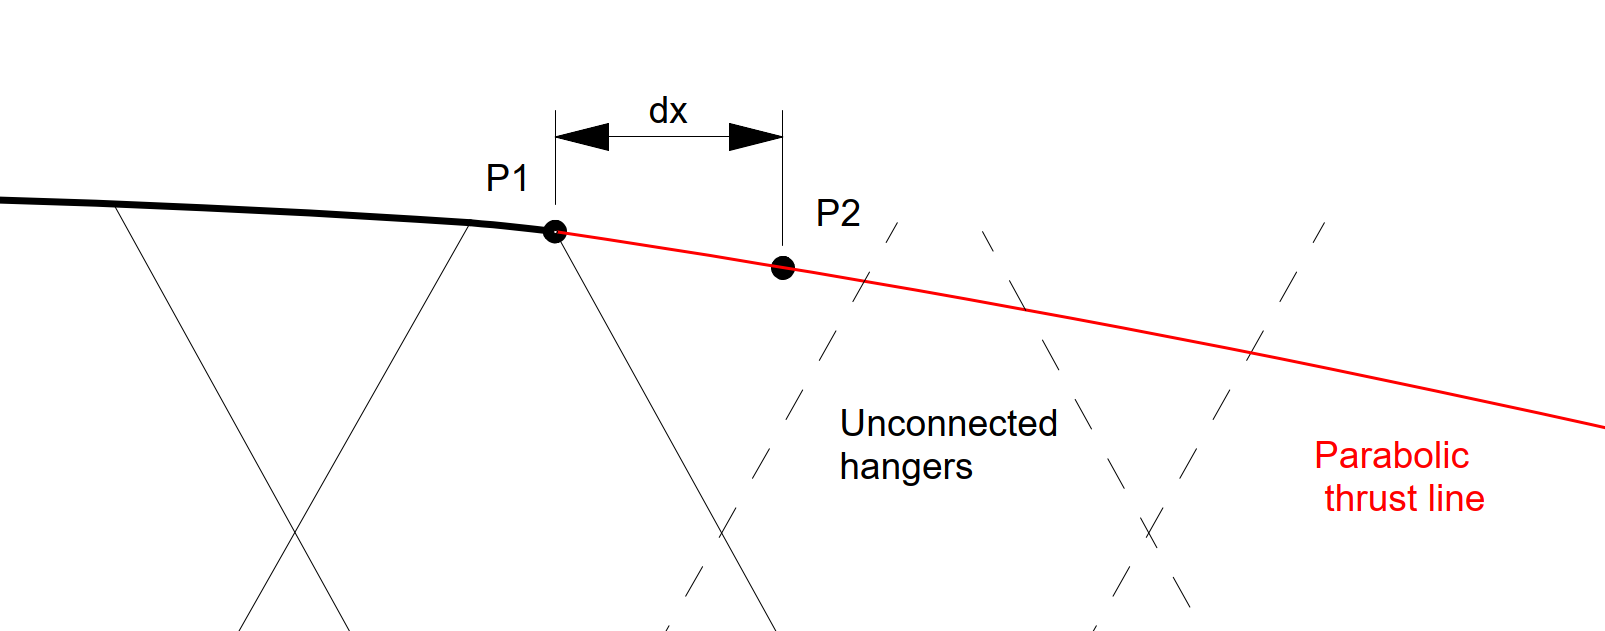
\includegraphics[width=0.7\textwidth]{overleaf/Appendix/Pictures/discrete_thrust_line_1.PNG}
    \caption{Thrust line derivation step without intersecting hangers}
    \label{fig:discrete_1}
\end{figure}

However, if a hanger intersects the thrust line within the current step, this intersection point is added to the thrust line and used as a starting point for the next step. This step is illustrated in Fig. \ref{fig:discrete_2}.

\begin{figure}[H]
    \centering
    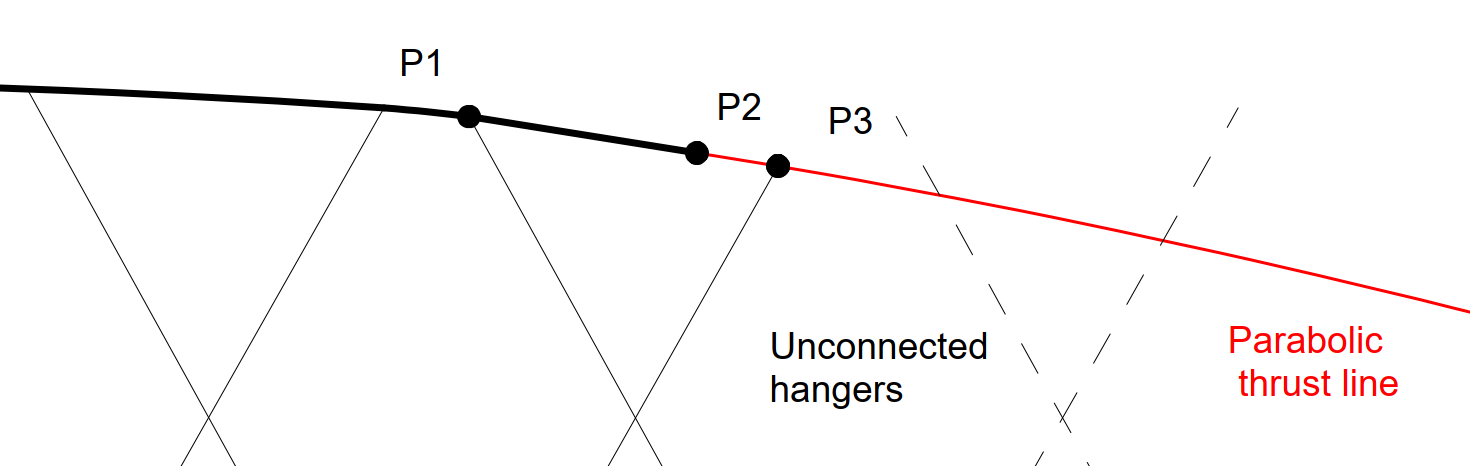
\includegraphics[width=0.7\textwidth]{overleaf/Appendix/Pictures/discrete_thrust_line_2.PNG}
    \caption{Thrust line derivation step connecting to the next hanger}
    \label{fig:discrete_2}
\end{figure}

Again, the normal force in the crown $N_{crown}$ is determined iteratively for the thrust line to intersect the knuckle point. Numerically, it would be much easier to calculate it from static considerations.

\section{Cost estimation}
In this chapter, the hanger unit costs are derived. The unit costs for the free length, the detailing and installation and the anchorages were received from a partner in the industry for \SI{150}{mm^2} strands and are given in Table \ref{tab:hanger_unit}.

\begin{table}[H]
\centering
\begin{tabular}{ccc}
\hline
Free length      & Detailing and installation & Anchorages    \\
3.00 \$/strand/m & 12.5 \$/strand/m           & 185 \$/strand \\ \hline
\end{tabular}
\caption{Hanger unit costs}
\label{tab:hanger_unit}
\end{table}

The total costs are calculated in Table \ref{tab:hanger_costs} for a single hanger set of the Blennerhassett Island Bridge. 

\begin{table}[H]
\centering
\resizebox{\textwidth}{!}{%
\begin{tabular}{lcccccc}
\hline
Hanger & Length  & Number of strands & Free length & Anchorage & Detailing and installation & Total cost \\
       & {[}m{]} & {[}-{]}           & {[}\${]}         & {[}\${]}       & {[}\${]}                   & {[}\${]}   \\ \hline
T1-H1  & 10.8    & 29                & \SI{938}{}              & \SI{5365}{}           & \SI{3907}{}                       & \SI{10210}{}      \\
T2-H2  & 21.5    & 29                & \SI{1868}{}             & \SI{5365}{}           & \SI{7784}{}                       & \SI{15017}{}      \\
T1-H3  & 24.1    & 29                & \SI{2097}{}             & \SI{5365}{}           & \SI{8738}{}                       & \SI{16201}{}      \\
T3-H4  & 31.3    & 29                & \SI{2721}{}             & \SI{5365}{}           & \SI{11339}{}                      & \SI{19425}{}      \\
T2-H5  & 38.3    & 29                & \SI{3332}{}             & \SI{5365}{}           & \SI{13882}{}                      & \SI{22579}{}      \\
T4-H6  & 39.8    & 29                & \SI{3461}{}             & \SI{5365}{}           & \SI{14421}{}                      & \SI{23247}{}      \\
TS-H7  & 46.9    & 29                & \SI{4083}{}             & \SI{5365}{}           & \SI{17012}{}                      & \SI{26460}{}      \\
T3-H8  & 48.8    & 29                & \SI{4245}{}             & \SI{5365}{}           & \SI{17686}{}                      & \SI{27295}{}      \\
T6-H9  & 52.6    & 29                & \SI{4574}{}             & \SI{5365}{}           & \SI{19059}{}                      & \SI{28998}{}      \\
T4-H10 & 55.1    & 29                & \SI{4797}{}             & \SI{5365}{}           & \SI{19986}{}                      & \SI{30147}{}      \\
T7-H11 & 56.5    & 29                & \SI{4917}{}             & \SI{5365}{}           & \SI{20488}{}                      & \SI{30770}{}      \\
TS-H12 & 58.2    & 29                & \SI{5061}{}             & \SI{5365}{}           & \SI{21087}{}                      & \SI{31512}{}      \\
T8-H13 & 58.5    & 29                & \SI{5088}{}             & \SI{5365}{}           & \SI{21201}{}                      & \SI{31654}{}      \\ \hline
Total  & 542.3   &                   & \SI{47181}{}            & \SI{69745}{}          & \SI{196588}{}                     & \SI{313515}{}     \\ \hline
\end{tabular}
}
\caption{Cost analysis for a hanger set of the Blennerhassett Island Bridge}
\label{tab:hanger_costs}
\end{table}

The costs per kilogram are determined in Eq. \ref{eq:hanger_unit_cost}, considering the hanger weight of \SI{31.9}{kg/m} and the area of \SI{140}{mm^2} per strand used in the Blennerhassett Island Bridge.

\begin{equation}
    \frac{\SI{313515}{\$}}{\SI{542.3}{m} \cdot \SI{31.9}{kg/m}} \, \frac{\SI{140}{mm^2}}{\SI{150}{mm^2}}= \SI{16.9}{\$/kg}
    \label{eq:hanger_unit_cost}
\end{equation}

\newpage
\section{Implementation}

